\documentclass[aspectratio=43,10pt]{beamer}

\usetheme[progressbar=frametitle]{metropolis}
\usepackage{appendixnumberbeamer}
\usepackage[ngerman]{babel}
\usepackage[utf8]{inputenc}
\usepackage{t1enc}

\usepackage{booktabs}
\usepackage[scale=2]{ccicons}
\usepackage{hyperref}

\usepackage{pgf}
\usepackage{tikz}
\usetikzlibrary{arrows,automata,positioning}
\usepackage{pgfplots}
\usepgfplotslibrary{dateplot}

\usepackage{xspace}
\newcommand{\themename}{\textbf{\textsc{metropolis}}\xspace}

\usepackage{blindtext}
\usepackage{graphicx}
\usepackage{subcaption}
\usepackage{comment}
\usepackage{mathtools}
\usepackage{amsmath}
\usepackage{centernot}
\usepackage{amssymb}
\usepackage{proof}
\usepackage{tabularx}
\renewcommand{\figurename}{Abb.}
\usepackage{marvosym}
\usepackage{mathtools}
\usepackage{qrcode}

\definecolor{ExColor}{HTML}{17819b}

\newcommand{\emptyWord}{\varepsilon}
\newcommand{\SigmaStern}{\Sigma^{*}}
\newcommand{\absval}[1]{|#1|}
\newcommand{\defeq}{\vcentcolon=}
\newcommand{\eqdef}{=\vcentcolon}
\newcommand{\nimplies}{\centernot\implies}

\newcommand{\naturals}{\ensuremath{\mathbb{N}}}
\newcommand{\integers}{\ensuremath{\mathbb{Z}}}
\newcommand{\rationals}{\ensuremath{\mathbb{Q}}}
\newcommand{\reals}{\ensuremath{\mathbb{R}}}

\setbeamertemplate{footline}[text line]
{\parbox{\linewidth}{Fachgruppe Informatik\hfill\insertpagenumber\hfill Vorkurs Theoretische Informatik\vspace{0.2in}}}


\title{Vorkurs Theoretische Informatik}
\subtitle{Induktion und Einführung in die Grammatik}
\date{Mittwoch, 14.10.2020}
\author{Arbeitskreis Theo Vorkurs}
\institute{Fachgruppe Informatik}
% \titlegraphic{\hfill\includegraphics[height=1.5cm]{logo.pdf}}

\begin{document}

\maketitle

\begin{frame}[fragile]{Übersicht}
  \setbeamertemplate{section in toc}[sections numbered]
  \tableofcontents%[hideallsubsections]
\end{frame}

\section{Vollständige Induktion}

\subsubsection{Idee}
\begin{frame}[fragile]{Idee}
\begin{columns}
\column{0.5\textwidth}
    \begin{alertblock}{Zeige Aussagen der Form:\\\emph{Für alle $n\in\mathbb{N}$ gilt...}}
    \begin{enumerate}
        \item Zeige Aussage für das kleinste Element
        \item<1-> \only<7,8>{\alert<7>{Zeige, wenn Aussage für beliebiges n gilt, gilt sie auch für dessen Nachfolger, also n+1.}}\onslide<1-6>{Zeige, dass Aussage auch für das folgende Element gilt.}
        \item<2-6,8> \only<8>{\alert<8>{$\leadsto$ Aussage gilt für alle n.}}\onslide<2-6>{\small Zeige, dass Aussage auch für das folgende Element gilt.}
        \item<3-6> \footnotesize Zeige, dass Aussage auch für das folgende Element gilt.
        \item<4-6> \scriptsize Zeige, dass Aussage auch für das folgende Element gilt.
        \item<5-6> \tiny Zeige, dass Aussage auch für das folgende Element gilt.
        \item<6> \dots
    \end{enumerate}
    \end{alertblock}
\column{0.5\textwidth}
    \begin{figure}
        \centering
        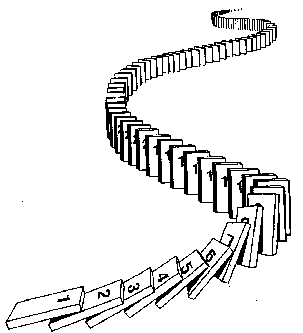
\includegraphics[width=0.7\textwidth]{../figures/induction.jpg}
        %\caption{Idee}
        %
    \end{figure}
\end{columns}
\end{frame}

\subsubsection{Funktionsweise}
\begin{frame}[fragile]{Struktur}
    \begin{alertblock}{Zeige Aussagen der Form:\\\emph{Für alle $n\in\mathbb{N}$ gilt...}}
    \begin{enumerate}
        \item \alert{Induktionsanfang}\\Zeige Aussage für das kleinste Element
        \item \alert{Induktionsvorraussetzung}\\Zeige, unter der Vorraussetzung: \\\emph{die Aussage gelte für beliebiges n},\dots
        \item \alert{Induktionsschritt}\\\dots dann gilt die Aussage auch für dessen Nachfolger n+1.
        \item $\leadsto$ Aussage gilt für alle $n \in \mathbb{N}$.
    \end{enumerate}
    \end{alertblock}
\end{frame}

\begin{frame}[fragile]{Beispiel}
\center $\displaystyle\sum_{i = 0}^{n} (2i+1) = (n+1)^2,\quad\forall n \in\mathbb{N}$.
    \begin{figure}
        \centering
        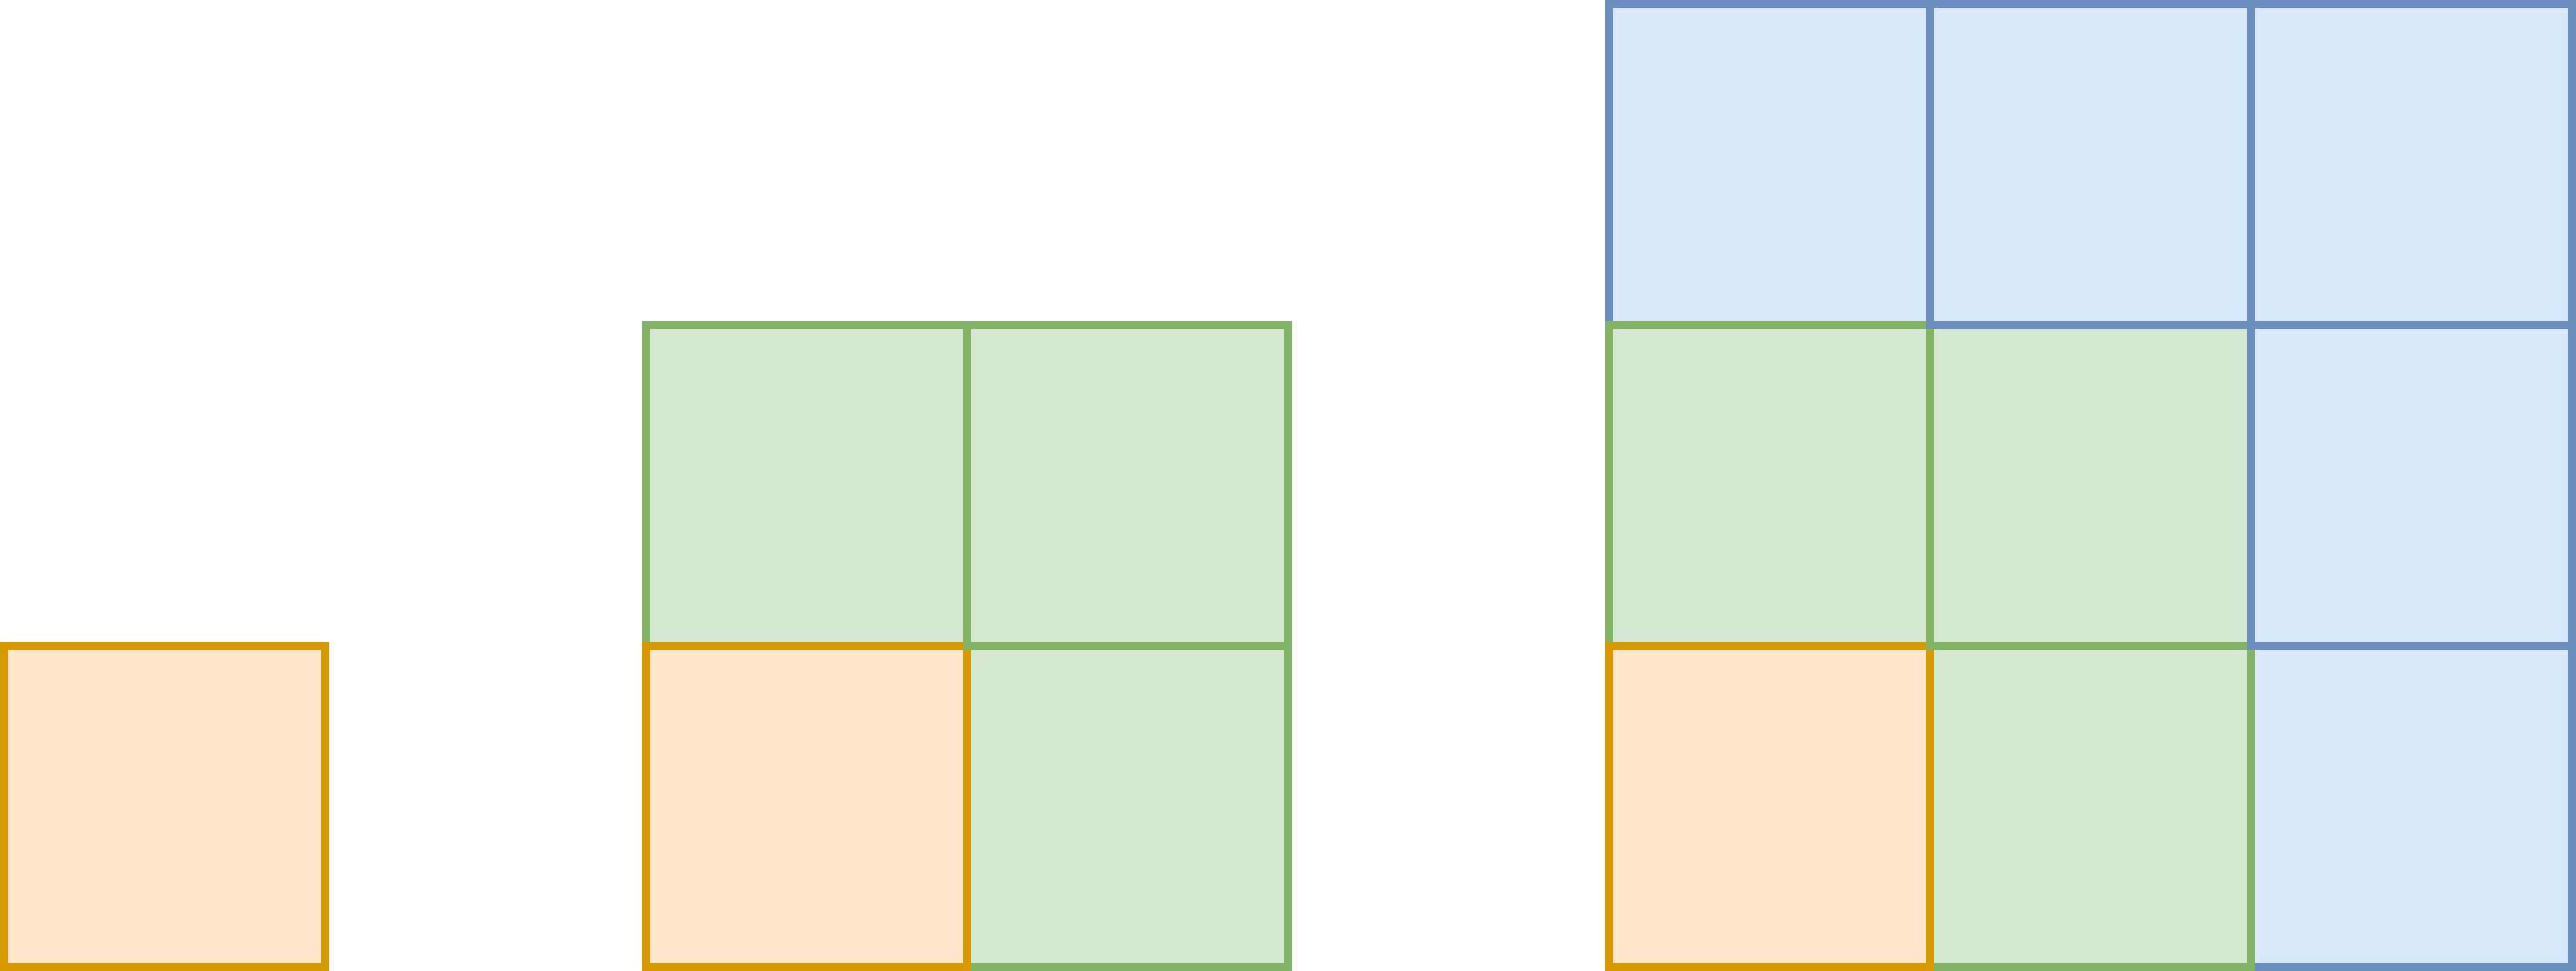
\includegraphics[width=0.5\textheight]{../figures/Summe.png}\qquad \dots
        %\caption{Idee}
        %
    \end{figure}
\end{frame}

\begin{frame}[fragile]{Beispiel}
Zeigen Sie $\displaystyle\sum_{i = 0}^{n} (2i+1) = (n+1)^2,\quad\forall n \in\mathbb{N}$.
\begin{alertblock}{Induktionsanfang IA}
    Zeige Aussage gilt für $n\defeq0$:\\
    \begin{align*}
        \sum_{i = 0}^{0} (2i+1) &\overset{!}{=} (0+1)^2\\
        \iff 2 * 0 + 1 &\overset{!}{=}1^2\\
        \iff 1 &= 1 \qquad\checkmark
    \end{align*}
\end{alertblock}
\end{frame}

\begin{frame}[fragile]{Beispiel}
Zeigen Sie $\displaystyle\sum_{i = 0}^{n} (2i+1) = (n+1)^2,\quad\forall n \in\mathbb{N}$.
\begin{alertblock}{Induktionsanfang IA}
    Aussage gilt für $n\defeq0$, da $\sum_{i = 0}^{0} (2i+1) = 0^2$
\end{alertblock}
\begin{alertblock}{Induktionsvorraussetzung IV}
    Ang. Aussage gilt für $n \in\mathbb{N}$.
\end{alertblock}
\begin{alertblock}{Induktionsschritt IS}
    Zeige Aussage gilt für alle n+1 unter Nutzung der I.V.:\\
    $\sum_{i = 0}^{\alert{n+1}} (2i+1) \overset{!}{=} (\alert{(n+1)}+1)^2$
\end{alertblock}
\end{frame}

\begin{frame}[fragile]{Beispiel}
\small\begin{alertblock}{Induktionsschritt}
    Zeige Aussage gilt für alle n+1 unter Nutzung der I.V.:
    \begin{align*}
        \onslide<1->{&\sum_{i = 0}^{n+1} (2i+1)&\overset{!}{=} ((n+1)+1)^2}\\
        \onslide<2->{\iff&\sum_{i = 0}^{\alert<2>{n}} (2i+1) + \sum_{i = \alert<2>{n+1}}^{n+1} (2i+1)&\overset{!}{=} (n+2)^2}\\
        \onslide<3->{\iff&\sum_{i = 0}^{n} (2i+1) + ( 2(n+1)+1 )&\overset{!}{=} n^2 + 2 * 2n + 2^2}\\
        \onslide<4->{\overset{\alert<4>{IV}}\iff&\alert<4>{(n+1)^2} + ( 2(n+1)+1 )&\overset{!}{=} n^2+4n+4}\\
        \onslide<5->{\iff&n^2+2n+1^2+2n+2+1&\overset{!}{=} n^2+4n+4}\\
        \onslide<6>{\iff&n^2+4n+4&\alert<6>{=} n^2+4n+4}
    \end{align*}
\end{alertblock}
\end{frame}

\begin{frame}[fragile]{Beispiel}
Zeigen Sie $\displaystyle\sum_{i = 0}^{n} (2i+1) = (n+1)^2,\quad\forall n \in\mathbb{N}$.
\begin{alertblock}{Induktionsanfang IA}
    Aussage gilt für $n\defeq0$, da $\sum_{i = 0}^{0} (2i+1) = 1^2$
\end{alertblock}
\begin{alertblock}{Induktionsvorraussetzung IV}
    Ang. Aussage gilt für alle $n \in\mathbb{N}$.
\end{alertblock}
\begin{alertblock}{Induktionsschritt IS}
    Aussage gilt für alle n+1 unter Nutzung der I.V., da\\
    $\sum_{i = 0}^{n+1} (2i+1) = ((n+1)+1)^2$
\end{alertblock}
\alert{$\leadsto$ Aussage gilt für alle n.}\qed
\end{frame}


{\setbeamercolor{palette primary}{bg=ExColor}
\begin{frame}[fragile]{Denkpause}
    \begin{alertblock}{Aufgaben}
    Versuche dich an den folgenden Induktionsbeweisen.
    \end{alertblock}
    
    \metroset{block=fill}
    \begin{block}{Normal}
        $\displaystyle\sum_{i=0}^{n} i = \frac{n(n+1)}{2}$, für alle $n \in \mathbb{N}$
    \end{block}
    \begin{block}{Schwerer}
        $\displaystyle\prod_{i=1}^{n} 4^i = 2^{n(n+1)}$, für alle $n \in \mathbb{N}\setminus \{0\}$
    \end{block}
\end{frame}
}

%\subsubsection{Lösungen normal}
{\setbeamercolor{palette primary}{bg=ExColor}
\begin{frame}[fragile]{Lösungen: normale Aufgabe}
    Zu zeigen: $\displaystyle\sum_{i=0}^{n} i = \frac{n(n+1)}{2}$ gilt für alle $n \in \mathbb{N}$.
    \begin{alertblock}{Induktionsanfang IA}
        Aussage gilt für $n\defeq 0$, da $\displaystyle\sum_{i=0}^{1} i = 0 = \frac{0(0+1)}{2}$.
    \end{alertblock}
    \begin{alertblock}{Induktionsvorraussetzung IV}
        Ang. Aussage gilt für $n \in\mathbb{N}$.
    \end{alertblock}
    \begin{alertblock}{Induktionsschritt IS}
        Zeige Aussage gilt für alle n+1 unter Nutzung der I.V.:\\
        $\displaystyle\sum_{i=0}^{\alert{n+1}} i \overset{!}{=} \frac{(\alert{n+1})((\alert{n+1})+1)}{2}$
    \end{alertblock}
\end{frame}


\begin{frame}[fragile]{Lösungen: normale Aufgabe}
\small\begin{alertblock}{Induktionsschritt}
    Zeige Aussage gilt für alle n+1 unter Nutzung der I.V.:
    \begin{align*}
        \onslide<1->{&\displaystyle\sum_{i=0}^{\alert<1>{n+1}} i &\overset{!}{=} \frac{(\alert<1>{n+1})((\alert<1>{n+1})+1)}{2}}\\
        \onslide<2->{\iff&(\displaystyle\sum_{i=0}^{n} i)+(n+1) &\overset{!}{=} \frac{(n+1)(n+2)}{2}}\\
        \onslide<3->{\iff&(\displaystyle\sum_{i=0}^{n} i)+(n+1) &\overset{!}{=} \frac{n^2+3n+2}{2}}\\
        \onslide<4->{\overset{\alert<4>{IV}}\iff&\alert<4>{\frac{n(n+1)}{2}}+(n+1) &\overset{!}{=} \frac{n^2+3n+2}{2}}\\
        \onslide<5->{\iff&\frac{n^2+n}{2}+\frac{2n+2}{2} &\overset{!}{=} \frac{n^2+3n+2}{2}}\\
        \onslide<6->{\iff&\frac{n^2+3n+2}{2} &\alert{=} \frac{n^2+3n+2}{2}}\\
    \end{align*}
\end{alertblock}
\end{frame}


\begin{frame}[fragile]{Lösungen: normale Aufgabe}
    Zu zeigen: $\displaystyle\sum_{i=0}^{n} i = \frac{n(n+1)}{2}$ gilt für alle $n \in \mathbb{N}$.
    \begin{alertblock}{Induktionsanfang IA}
        Aussage gilt für $n\defeq 0$, da $\displaystyle\sum_{i=0}^{1} i = 0 = \frac{0(0+1)}{2}$.
    \end{alertblock}
    \begin{alertblock}{Induktionsvorraussetzung IV}
        Ang. Aussage gilt für $n \in\mathbb{N}$.
    \end{alertblock}
    \begin{alertblock}{Induktionsschritt IS}
        Zeige Aussage gilt für alle n+1 unter Nutzung der I.V.:\\
        $\displaystyle\sum_{i=0}^{\alert{n+1}} i \overset{!}{=} \frac{(\alert{n+1})((\alert{n+1})+1)}{2}$ gilt für alle $n \in \mathbb{N}$
    \end{alertblock}
    \alert{$\leadsto$ Aussage gilt für alle n.}\qed
\end{frame}
}

% \begin{frame}[standout]
%   Fragen dazu?
% \end{frame}

%\subsubsection{Lösungen schwerer}
{\setbeamercolor{palette primary}{bg=ExColor}
\begin{frame}[fragile]{Lösungen: schwerere Aufgabe}
    Zu zeigen: $\displaystyle\prod_{i=1}^{n} 4^i = 2^{n(n+1)}$, für alle $n \in \mathbb{N}\setminus \{0\}$.
    \begin{alertblock}{Induktionsanfang IA}
        Aussage gilt für $n\defeq 1$, da $\displaystyle\prod_{i=1}^{1} 4^i = 4^1 = 4 = 2^2 = 2^{1(1+1)}$.
    \end{alertblock}
    \begin{alertblock}{Induktionsvorraussetzung IV}
        Ang. Aussage gilt für $n \in\mathbb{N}\setminus \{0\}$.
    \end{alertblock}
    \begin{alertblock}{Induktionsschritt IS}
        Zeige Aussage gilt für alle n+1 unter Nutzung der I.V.:\\
        $\displaystyle\prod_{i=1}^{\alert{n+1}} 4^i \overset{!}{=} 2^{(\alert{n+1})((\alert{n+1})+1)}$
    \end{alertblock}
\end{frame}

\begin{frame}[fragile]{Lösungen: schwerere Aufgabe}
\small\begin{alertblock}{Induktionsschritt}
    Zeige Aussage gilt für alle n+1 unter Nutzung der I.V.:
    \begin{align*}
        \onslide<1->{&\displaystyle\prod_{i=1}^{\alert<1>{n+1}} 4^i &\overset{!}{=} 2^{(\alert<1>{n+1})((\alert<1>{n+1})+1)}}\\
        \onslide<2->{\iff&(\displaystyle\prod_{i=1}^{n} 4^i) * 4^{(n+1)} &\overset{!}{=} 2^{(n+1)(n+2)}}\\
        \onslide<3->{\overset{\alert<3>{IV}}\iff&\alert<3>{(2^{n(n+1)})} * 4^{(n+1)} &\overset{!}{=} 2^{n^2+3n+2}}\\
        \onslide<4->{\iff&2^{n^2+n} * 2^{2(n+1)} &\overset{!}{=} 2^{n^2+3n+2}}\\
        \onslide<5->{\iff&2^{n^2+n} * 2^{2n+2} &\overset{!}{=} 2^{n^2+3n+2}}\\
        \onslide<6->{\iff&2^{(n^2+n)+(2n+2)} &\overset{!}{=} 2^{n^2+3n+2}}\\
        \onslide<7->{\iff&2^{n^2+3n+3} &\alert{=} 2^{n^2+3n+2}}
    \end{align*}
\end{alertblock}
\end{frame}


\begin{frame}[fragile]{Lösungen: schwerere Aufgabe}
     Zu zeigen: $\displaystyle\prod_{i=1}^{n} 4^i = 2^{n(n+1)}$, für alle $n \in \mathbb{N}\setminus \{0\}$.
    \begin{alertblock}{Induktionsanfang IA}
        Aussage gilt für $n\defeq 1$, da $\displaystyle\prod_{i=1}^{1} 4^i = 4^1 = 4 = 2^2 = 2^{1(1+1)}$.
    \end{alertblock}
    \begin{alertblock}{Induktionsvorraussetzung IV}
        Ang. Aussage gilt für $n \in\mathbb{N}\setminus \{0\}$.
    \end{alertblock}
    \begin{alertblock}{Induktionsschritt IS}
        Zeige Aussage gilt für alle n+1 unter Nutzung der I.V.:\\
        $\displaystyle\prod_{i=1}^{\alert{n+1}} 4^i \overset{!}{=} 2^{(\alert{n+1})((\alert{n+1})+1)}$ gilt für alle $n \in \mathbb{N}\setminus \{0\}$
    \end{alertblock}
    \alert{$\leadsto$ Aussage gilt für alle n.}\qed
\end{frame}
}

% \begin{frame}[standout]
%   Fragen dazu?
% \end{frame}


\begin{frame}[standout]
  Murmelpause
\end{frame}

%Vollständige Induktion aus Tag 2
% \section{Wiederholung: Vollständige Induktion}

% \subsection{Definition}

% \begin{frame}[fragile]{Definition}
%     \begin{enumerate}
%         \item \textbf{Induktionsanfang} (Gilt die Aussage für ein $n_0$) \\
%         \item \textbf{Induktionsvoraussetzung} (wir nehmen dann an, die Aussage gilt tatsächlich)
%         \item \textbf{Induktionsschritt} (Hier zeigen wir, dass für alle $n \in \mathbb{N}$ die Aussage gilt, unter Verwendung der IV)
%     \end{enumerate}
% \end{frame}

\subsubsection{formalere Definition}
\begin{frame}{Definition nochmal formaler}
    \begin{equation*}
        (\forall n \in \mathbb{N}_{n_0}: P(n)) \iff (P(n_0) \wedge \forall n \in \mathbb{N}_{n_0}: (P(n) \implies P(n+1)))
    \end{equation*}    
\end{frame}

\begin{frame}{Definition nochmal formaler}
    \onslide<1->$(\forall n \in \mathbb{N}_{n_0}: P(n)) \iff (\alert<2>{\underbrace{P(n_0)}_{\text{IA}}}\wedge \overbrace{\alert<3>{\forall n \in \mathbb{N}_{n_0}:} (\alert<4>{\underbrace{P(n)}_{\text{IV}}} \alert<5>{\implies P(n+1)})}^{\text{IS}})$
    \begin{enumerate}
        \item<2->\alert<2>{\textbf{IA:} $n = n_0$}
        \item<3->\onslide<3->{\alert<3>{\textbf{IS:} Sei $n\in\mathbb{N}_{n_0}$ beliebig.}}
        \onslide<4->{\alert<4>{Ang. es gilt $P(n)$. \tiny{\textbf{(IV)}}}}    
        \item<5->\alert{$\leadsto$ Zeigen, dass $P(n+1)$ gilt, unter Verwendung von $P(n)$ \tiny{\textbf{(IV)}}}
    \end{enumerate}
\end{frame}

% \begin{frame}{Aufgabe zur Wiederholung}
%     Warum das ganze nur für Summen.\\
%     Angenommen $n^3-n$ ist durch 3 teilbar für alle natürlichen Zahlen.\\
%     Wie gehen wir dann hier vor?
% \end{frame}

% \begin{frame}{Aufgabe zur Wiederholung}
%     \begin{itemize}
%         \item<1->
%             Schreiben wir das ganze erst mal etwas Mathematischer.
%         \item<2->
%             $3 \mid n^3-n$, also 3 teilt $n^3-n$
%         \item<3->
%             Jetzt vollständige Induktion
%     \end{itemize}
% \end{frame}

% \begin{frame}{Vollständige Induktion}
%     \begin{enumerate}
%         \item<1->
%             \textbf{IA:} n = 1
%                 \begin{equation*}
%                     3 \mid 1^3 - 1 \iff 3 \mid 1 - 1 \iff 3 \mid 0 \qquad \checkmark
%                 \end{equation*}
%         \item<2->
%             % \textbf{IV:}\\
%             % Da $3 \mid n^3-n$ für 1 gilt, existiert also eine Zahl $n\in \mathbb{N}$ (beliebig aus den natürlichen Zahlen, hier 1 da wir es bereits dafür gezeigt haben), für welche die Aussage $3 \mid n^3 -n$ gilt.
%              \textbf{IS:} Sei $n \in \mathbb{N}$ beliebig. Ang., es gilt $3\mid n^3-n$ (IV)
%             \begin{align*}
%                 3 \mid (n+1)^3-(n+1) &\iff 3\mid(n+1)^3 - n - 1\\
%                 &\iff 3\mid n^3 + 3n^2 + 3n + 1 - n - 1\\
%                 &\iff 3\mid \underbrace{n^3 - n}_{\text{Induktionsvoraussetzung}} + \underbrace{3n^2 + 3n}_{\text{vielfache von 3}} + \underbrace{1 - 1}_{= 0}\\
%                 &\iff 3\mid(n^3 - n) + 3(n^2 + n)
%             \end{align*}
%         \item<3->
%         \textbf{Fazit:}\\
%             Nach Voraussetzung ist der erste Summand durch 3 teilbar, und der zweite Summand ist ein vielfaches von 3. Somit ist auch die Summe durch 3 teilbar.
%     \end{enumerate}    
% \end{frame}

% \begin{frame}[fragile]{Ein Aufgabe zur Übung}
%     \begin{itemize}
%         \item Zeigen Sie, dass für alle natürlichen Zahlen $n \geq 4$ gilt: \\
%         \begin{center}
%             $n! > 2^n$\\
%         \end{center}
%     \end{itemize}
% \end{frame}

% {\setbeamercolor{palette primary}{bg=ExColor}
% \begin{frame}{Lösung}
%     \begin{enumerate}
%         \item 
%             \textbf{IA:} n = 4
%             \begin{equation*}
%                 4! = 4 \cdot 3 \cdot 2 \cdot 1 = 24 > 16 = 2^4
%             \end{equation*}
%         \item    
%             \textbf{IV:}
%             Die Aussage $n! > 2^n$ gilt für n=4, also existiert ein $x\in \mathbb{N}$, sodass diese Aussage gilt.
%         \item    
%             \textbf{IS:} Also gilt die Aussage für n+1
%             \begin{align*}
%                 (n+1)! &= (n+1) \cdot n!\\
%                 &\overset{\text{nach IV.}}{>} \underbrace{(n+1)}_{\text{da n min. 4}} \cdot 2^n\\
%                 &\overset{(n+1)>2}{>} 2 \cdot 2^n = 2^{n+1}
%             \end{align*}
%         \item
%             \textbf{Fazit:}\\
%             Somit ist für alle $n\in \mathbb{N}$(beliebige natürliche Zahl) gezeigt, dass $n! > 2^n$ für $n \geq 4$.
%     \end{enumerate}
% \end{frame}
% }

% %An der Tafel die Lösung besprechen 


{\setbeamercolor{palette primary}{bg=ExColor}
	\begin{frame}[fragile]{Aufgabe}
		\metroset{block=fill}
		\begin{alertblock}{Die folgende Induktion zeigt eine seltsame Aussage.}
			Ist der Beweis korrekt geführt? Was ist passiert?
		\end{alertblock}
		\metroset{block=transparent}
		Sei $A(n)\defeq$ In einer Herde aus $n$ Telefonen haben alle die selbe Farbe.
		Zu zeigen: $A(n)$ gilt für alle $n \in \mathbb{N}^+$.
		\begin{alertblock}{Induktionsanfang IA}
			$A(1)$: Aussage gilt für $n\defeq 1$, da ein Telefon nur eine Farbe haben kann.
		\end{alertblock}
		\begin{alertblock}{Induktionsvorraussetzung IV}
			Ang. $A(n)$ gilt für $n\geq1$.
		\end{alertblock}
		\begin{alertblock}{Induktionsschritt IS}
			Zeige Aussage gilt für alle $n+1$ unter Nutzung der I.V.\\
			d.h. wir zeigen $A(n+1)=$ In einer Herde aus $n+1$ Telefonen haben alle die selbe Farbe.
		\end{alertblock}
	\end{frame}
	\begin{frame}[fragile]{Aufgabe}
		\footnotesize{
			\begin{alertblock}{Induktionsschritt IS}
				Wir betrachten eine Herde aus $n+1$ Telefonen:
				\[\underbrace{\text{\Telefon}\text{\Telefon}\text{\Telefon}\text{\Telefon}\text{\Telefon}\dots\text{\Telefon}\text{\Telefon}}_{n+1}\]
				Wir sondern ein Telefon aus und betrachten den Rest. Nach I.V. haben diese alle die selbe Farbe.
				\[\underbrace{\alert{\text{\Telefon}\text{\Telefon}\text{\Telefon}\text{\Telefon}\text{\Telefon}\dots\text{\Telefon}}}_{n}\text{\Telefon}\]
				Jetzt sondern wir ein anderes Telefon aus.
				\[\alert{\text{\Telefon}}\underbrace{\alert{\text{\Telefon}\text{\Telefon}\text{\Telefon}\text{\Telefon}\dots\text{\Telefon}}\text{\Telefon}}_{n}\]
				Die übrigen $n$ Telefone haben nach I.V. wieder die selbe Farbe.
				\[\underbrace{\alert{\text{\Telefon}\text{\Telefon}\text{\Telefon}\text{\Telefon}\text{\Telefon}\dots\text{\Telefon}\text{\Telefon}}}_{n+1}\]
				Also haben alle $n+1$ Telefone die selbe Farbe.
				$\leadsto$ $A(n)$ gilt für alle $n$.
			\end{alertblock}
		}
	\end{frame}
}

{\setbeamercolor{palette primary}{bg=ExColor}
	\begin{frame}[fragile]{Lösungen}
		\small{
			\metroset{block=fill}
			\begin{block}{Das Problem}
				Die Vorangehensweise erfordert, dass die betrachteten Mengen an $n$ Telefonen mindestens ein gemeinsames Element haben. Sie teilen dann die Farbe dieses Elements. Allerdings gibt es ein überlappendes Element erst ab $3$ Telefonen.
				\[
					\color{mLightGreen}A(1) \overset{\text{I.V.}}{\implies}
					\alert{A(2):\overbrace{\text{\Telefon}}\underbrace{\text{\Telefon}}} \color{black} \overset{\alert{\text{I.V.}}}{\nimplies}
					A(3):\rlap{$\overbrace{\phantom{\text{\Telefon\Telefon}}}$}\text{\Telefon}\underbrace{\text{\Telefon\Telefon}} 
					\overset{\alert{\text{I.V.}}}{\nimplies} \dots \overset{\alert{\text{I.V.}}}{\nimplies} A(n)
				\]
				Die Kette an verifiziert wahren Aussagen ist also unterbrochen, da es keine gültige Vorraussetzung gibt um $A(2+1)$ zu zeigen.
			\end{block}
		}
	
		\begin{figure}
		\resizebox{.6\textwidth}{!}{
			\centering%
			\begin{subfigure}{0.3\textwidth}
				\centering%
				
\includegraphics[height=0.5in]{../figures/green.jpg}
				\caption{grünes Telefon}
			\end{subfigure}
			$\qquad$
			\begin{subfigure}{0.3\textwidth}
				\centering%
				
\includegraphics[height=0.5in]{../figures/white.jpg}
				\caption{weißes Telefon}
			\end{subfigure}
		}
			\caption{Telefone mit unterschiedlicher Farbe\footnote{\tiny{Quelle: https://commons.wikimedia.org/}}}
		\end{figure}
	\end{frame}
}

\begin{frame}[standout]
  Murmelpause
\end{frame}

\section{Grammatiken}

\begin{frame}[fragile]{Wörter in Sprachen}
Wir können inzwischen Sprachen in Mengenschreibweise darstellen.\\Aber welche Wörter sind enthalten?\\
\vspace{0.3cm}
Wir können weitere Regeln formulieren, mit denen wir von einem gegebenen Startpunkt aus alle Wörter einer Sprache erzeugen können.
\end{frame}

\begin{frame}[fragile]{Beispiel Worterzeugung}
    \small{Wir betrachten L = \{$ww^R\;|\;w^R\text{ ist w rückwärts, }w \in \{a, b\}^n, n>0, n\in \mathbb{N}$\}\\
    Hier ist z.B. $\alert<1>{w}w^R$ = \alert<1>{ababb}bbaba $\in$ L.}\\
    \begin{enumerate}
    \item <2-> 
            \alert<2,5>{Wir beginnen mit einer Variablen S}
    \item <3-> 
            \alert<3>{Wir formulieren Regeln um S umzuwandeln}
            \alert<4>{\onslide<4->{
            \begin{align*}\alert<6,8>{S \rightarrow aSa}&\text{ oder }\alert<7,9>{S \rightarrow bSb}\\\text{oder }S \rightarrow aa &\text{ oder }\alert<10>{S \rightarrow bb}\end{align*}}}\vspace{-0.3in}
    \item <5->
            \alert<5>{Damit können wir jetzt Wörter aus der Sprache beschreiben.}\\
            z.B.: \alert<6>{a}\alert<7>{b}\alert<8>{a}\alert<9>{b}\alert<10>{bb}\alert<9>{b}\alert<8>{a}\alert<7>{b}\alert<6>{a} $\leadsto$ \only<5>{\alert<5>{S}}\only<6>{\alert<6>{aSa}}\only<7>{a\alert<7>{bSb}a}\only<8>{ab\alert<8>{aSa}ba}\only<9>{aba\alert<9>{bSb}aba}\only<10->{abab\alert<10>{bb}baba}
    \item <11> \alert<11>{Wir nennen diese Umformungsregeln Produktionsregeln.}
    \end{enumerate}
\end{frame}

\subsubsection{Produktionsregeln}
\begin{frame}{Produktionsregeln}
    \begin{alertblock}{Einschränkungen}
    \begin{itemize}
        \item \alert{\emph{Nichtterminale}} werden meist durch Großbuchstaben repräsentiert und müssen durch Produktionsregeln abgeändert werden
        \item \alert{\emph{Terminale}} werden meist durch Kleinbuchstaben repräsentiert und sollten \emph{nicht} durch weitere Produktionsregeln abgeändert werden
        \item Mehrere Symbole können auf einen Schlag überführt werden. Dabei sollten die Terminale nicht entfernt oder umsortiert werden.\\
        z.B. $AB \rightarrow CD$ ist erlaubt.\\
        Auch $abAB \rightarrow BbAa$, aber das gehört sich nicht.
    \end{itemize}
    \end{alertblock}
\end{frame}

\begin{frame}{Weitere Beispiele für Produktionen}
    \begin{alertblock}{Aufgaben}
    Gesucht: Produktionsregeln für die folgenden Sprachen.
    \end{alertblock}
    \metroset{block=fill}
    \begin{exampleblock}{$L_1 = \{a\}^*$}
    $\onslide<2->{P=\{S \rightarrow aS \only<3->{\mid \emptyWord}\}}$
    \end{exampleblock}
    \only<4->{
    \begin{exampleblock}{$L_2 = \{a, b\}^*$}
    $\onslide<5->{P=\{S \rightarrow  aS \only<6->{\mid bS}\only<7->{\mid \emptyWord}\}}$
    \end{exampleblock}
    }
\end{frame}

{\setbeamercolor{palette primary}{bg=ExColor}
\begin{frame}{Denkpause}
    \begin{alertblock}{Aufgaben}
    Findet Produktionsregeln für die folgenden Sprachen.
    \end{alertblock}
    \metroset{block=fill}
    \begin{block}{Normal}
    \begin{itemize}
        \item $L_1 = \{a^{2n}\;|\;n\in\mathbb{N}\}$
        \item $L_2 = \{a^nb^nc^m\;|\;n, m\in\mathbb{N}\}$
        \item $L_3 = \{uv\;|\;u\in\{a,b\}^\ast,\;v\in\{c,d\}\}$
        \item $L_4 = \{w\;|\;|w| = 3, w\in \{a,b,c\}^*\}$
    \end{itemize}
    \end{block}
    \begin{block}{Etwas Schwerer}
    \begin{itemize}
        \item $L_5 = \{a^n\;|\;n \equiv 1 \bmod 3\}$
        \item $L_6 = \{w\;|\;|w|_a = 3, |w|_b = 1, w\in \{a,b,c\}^*\}$
        \item $L_7 = \{uv\;|\;u\in\{\text{\Rewind, \MoveUp, \Forward, \MoveDown}\}^\ast,\;v\in\{\text{\Stopsign}\}\}$
        \item $L_8 = \{w\mid |w|=2, w \in \{a, b\}\}$
    \end{itemize}
    \end{block}
\end{frame}
}

{\setbeamercolor{palette primary}{bg=ExColor}
\begin{frame}{Lösungen}
Alle Lösungen sind Beispiellösungen, es sind auch andere möglich.
    \begin{itemize}
        \item<1-> \alert<1>{$P_1 = \{S\rightarrow aaS\;|\;\emptyWord$\}}
        \item<2-> \alert<2>{$P_2 = \{S\rightarrow AB$, $A\rightarrow aAb \;|\; ab\; |\;\emptyWord$, $B\rightarrow cB \;|\; \emptyWord$\}}
        \item<3-> \alert<3>{$P_3 = \{S\rightarrow UV$, $U\rightarrow aU \;|\; bU \; |\; \emptyWord$, $V\rightarrow c \;|\; d$\}}
        \item<4-> \alert<4>{$P_4 = \{S\rightarrow XXX$, $X\rightarrow a \;|\; b \;|\; c$\}}
        \item<5-> \alert<5>{$P_5 = \{S\rightarrow a \;|\; aaaS\}$}
        \item<6-> \alert<6>{$P_6 = \{S\rightarrow AAAB$, $AB\rightarrow BA$, 
        $A\rightarrow cA \;|\; Ac \;|\; a$, 
        $B\rightarrow cB \;|\; Bc \;|\; b$\}}
        \item<7-> \alert<7>{$P_7 = \{S\rightarrow U\text{\Stopsign} \;|\; \text{\Stopsign}$, $U\rightarrow \text{\Rewind} U \;|\; \text{\MoveUp} U \;|\; \text{\Forward} U \;|\; \text{\MoveDown} U \;|\;\emptyWord$\}}
        \item<8-> \alert<8>{$P_8 = \{\} \leadsto$ Es gibt keine Produktionsregeln!}
    \end{itemize}
\end{frame}
}  


\begin{frame}[standout]
  Murmelpause
\end{frame}

\subsubsection{formale Notation}
\begin{frame}[fragile]{Formale Notation}
    Wir beschreiben eine \alert{\emph{Grammatik}} durch ein geordentes \alert{\emph{Tupel}} $G = (V, \Sigma, P, S)$
    \begin{itemize}
        \item V ist die Menge der verwendeten Nichtterminale
        \item $\Sigma$ die Menge der Terminale bzw. unser Alphabet
        \item P ist die Menge der Produktionsregeln
        \item S ist die Startvariable
    \end{itemize}
    \metroset{block=fill}
    \begin{exampleblock}{Beispiel für  L = \{$ww^R\;|\;w^R\text{ ist w rückwärts, }w \in \{a, b\}^n, \; n \geq 1$\}}
        $G = (V,\Sigma,P,S)$, mit\\
        $V = \{S\}$\\
        $\Sigma = \{a,b\}$\\
        $P = \{S \rightarrow aSa, S \rightarrow bSb, S \rightarrow aa, S \rightarrow bb$\}\\
        \qquad bzw. kurz: $P = \{S \rightarrow aSa\;|\;bSb\;|\;aa\;|\;bb$\}
    \end{exampleblock}
\end{frame}

{\setbeamercolor{palette primary}{bg=ExColor}
\begin{frame}{Denkpause}
    \begin{columns}
\column{0.5\textwidth}
    \begin{alertblock}{knifflige Aufgabe}
    Bob will durch das Labyrinth laufen. Er hat folgende Möglichkeiten:\\
    $\Sigma$ = \{\text{\Rewind, \MoveUp, \Forward, \MoveDown}\}
    \begin{itemize}
        \item Bob kann nicht auf ein Feld zurücktreten von dem er gerade kam
        \item Bob geht bei jedem Schritt ein Feld in die angegebene Richtung
    \end{itemize}
    \end{alertblock}
\column{0.5\textwidth}
\begin{figure}
        \centering
        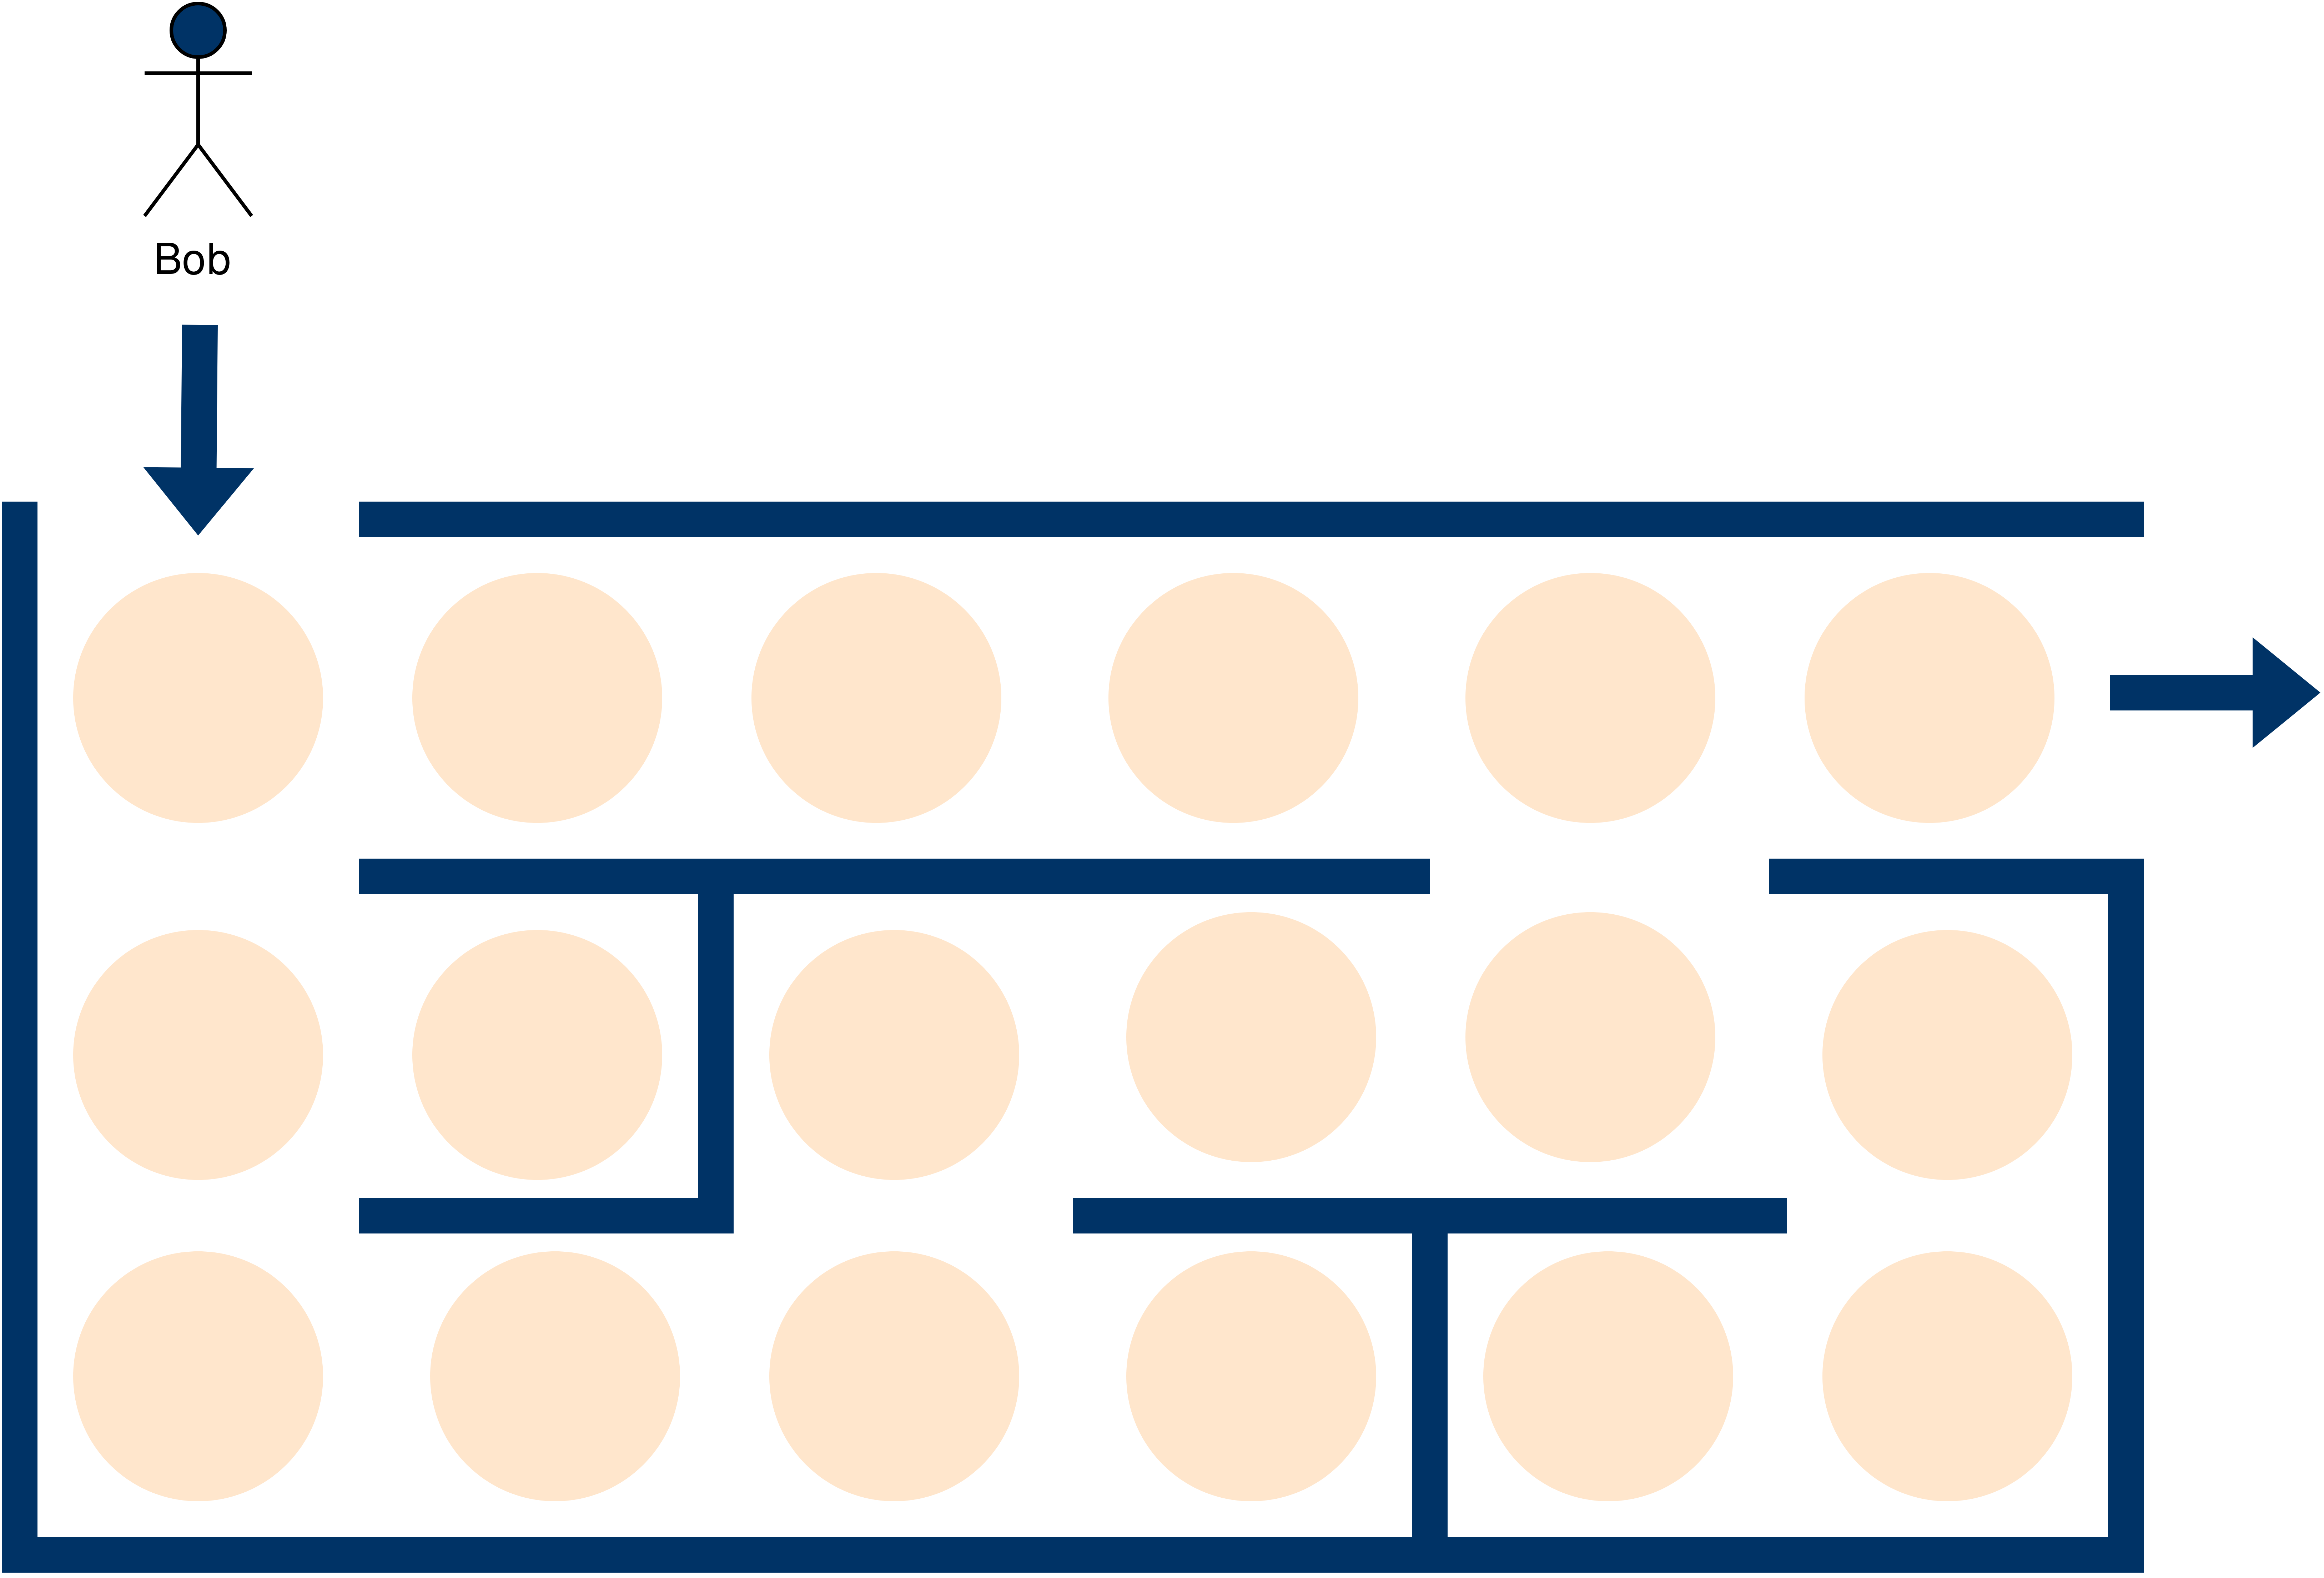
\includegraphics[width=0.7\textwidth]{../figures/GBeispiel.png}
        \caption{Bob's Problem}
        
    \end{figure}
\end{columns}
\alert{Geben Sie eine Grammatik an, welche die Sprache beschreibt, die Bob durch alle ihm möglichen Wege des Labyrinths führt.}
\end{frame}
}

{\setbeamercolor{palette primary}{bg=ExColor}
\begin{frame}{Denkpause}
    \begin{alertblock}{Beispiel}
    \begin{figure}
        \centering
        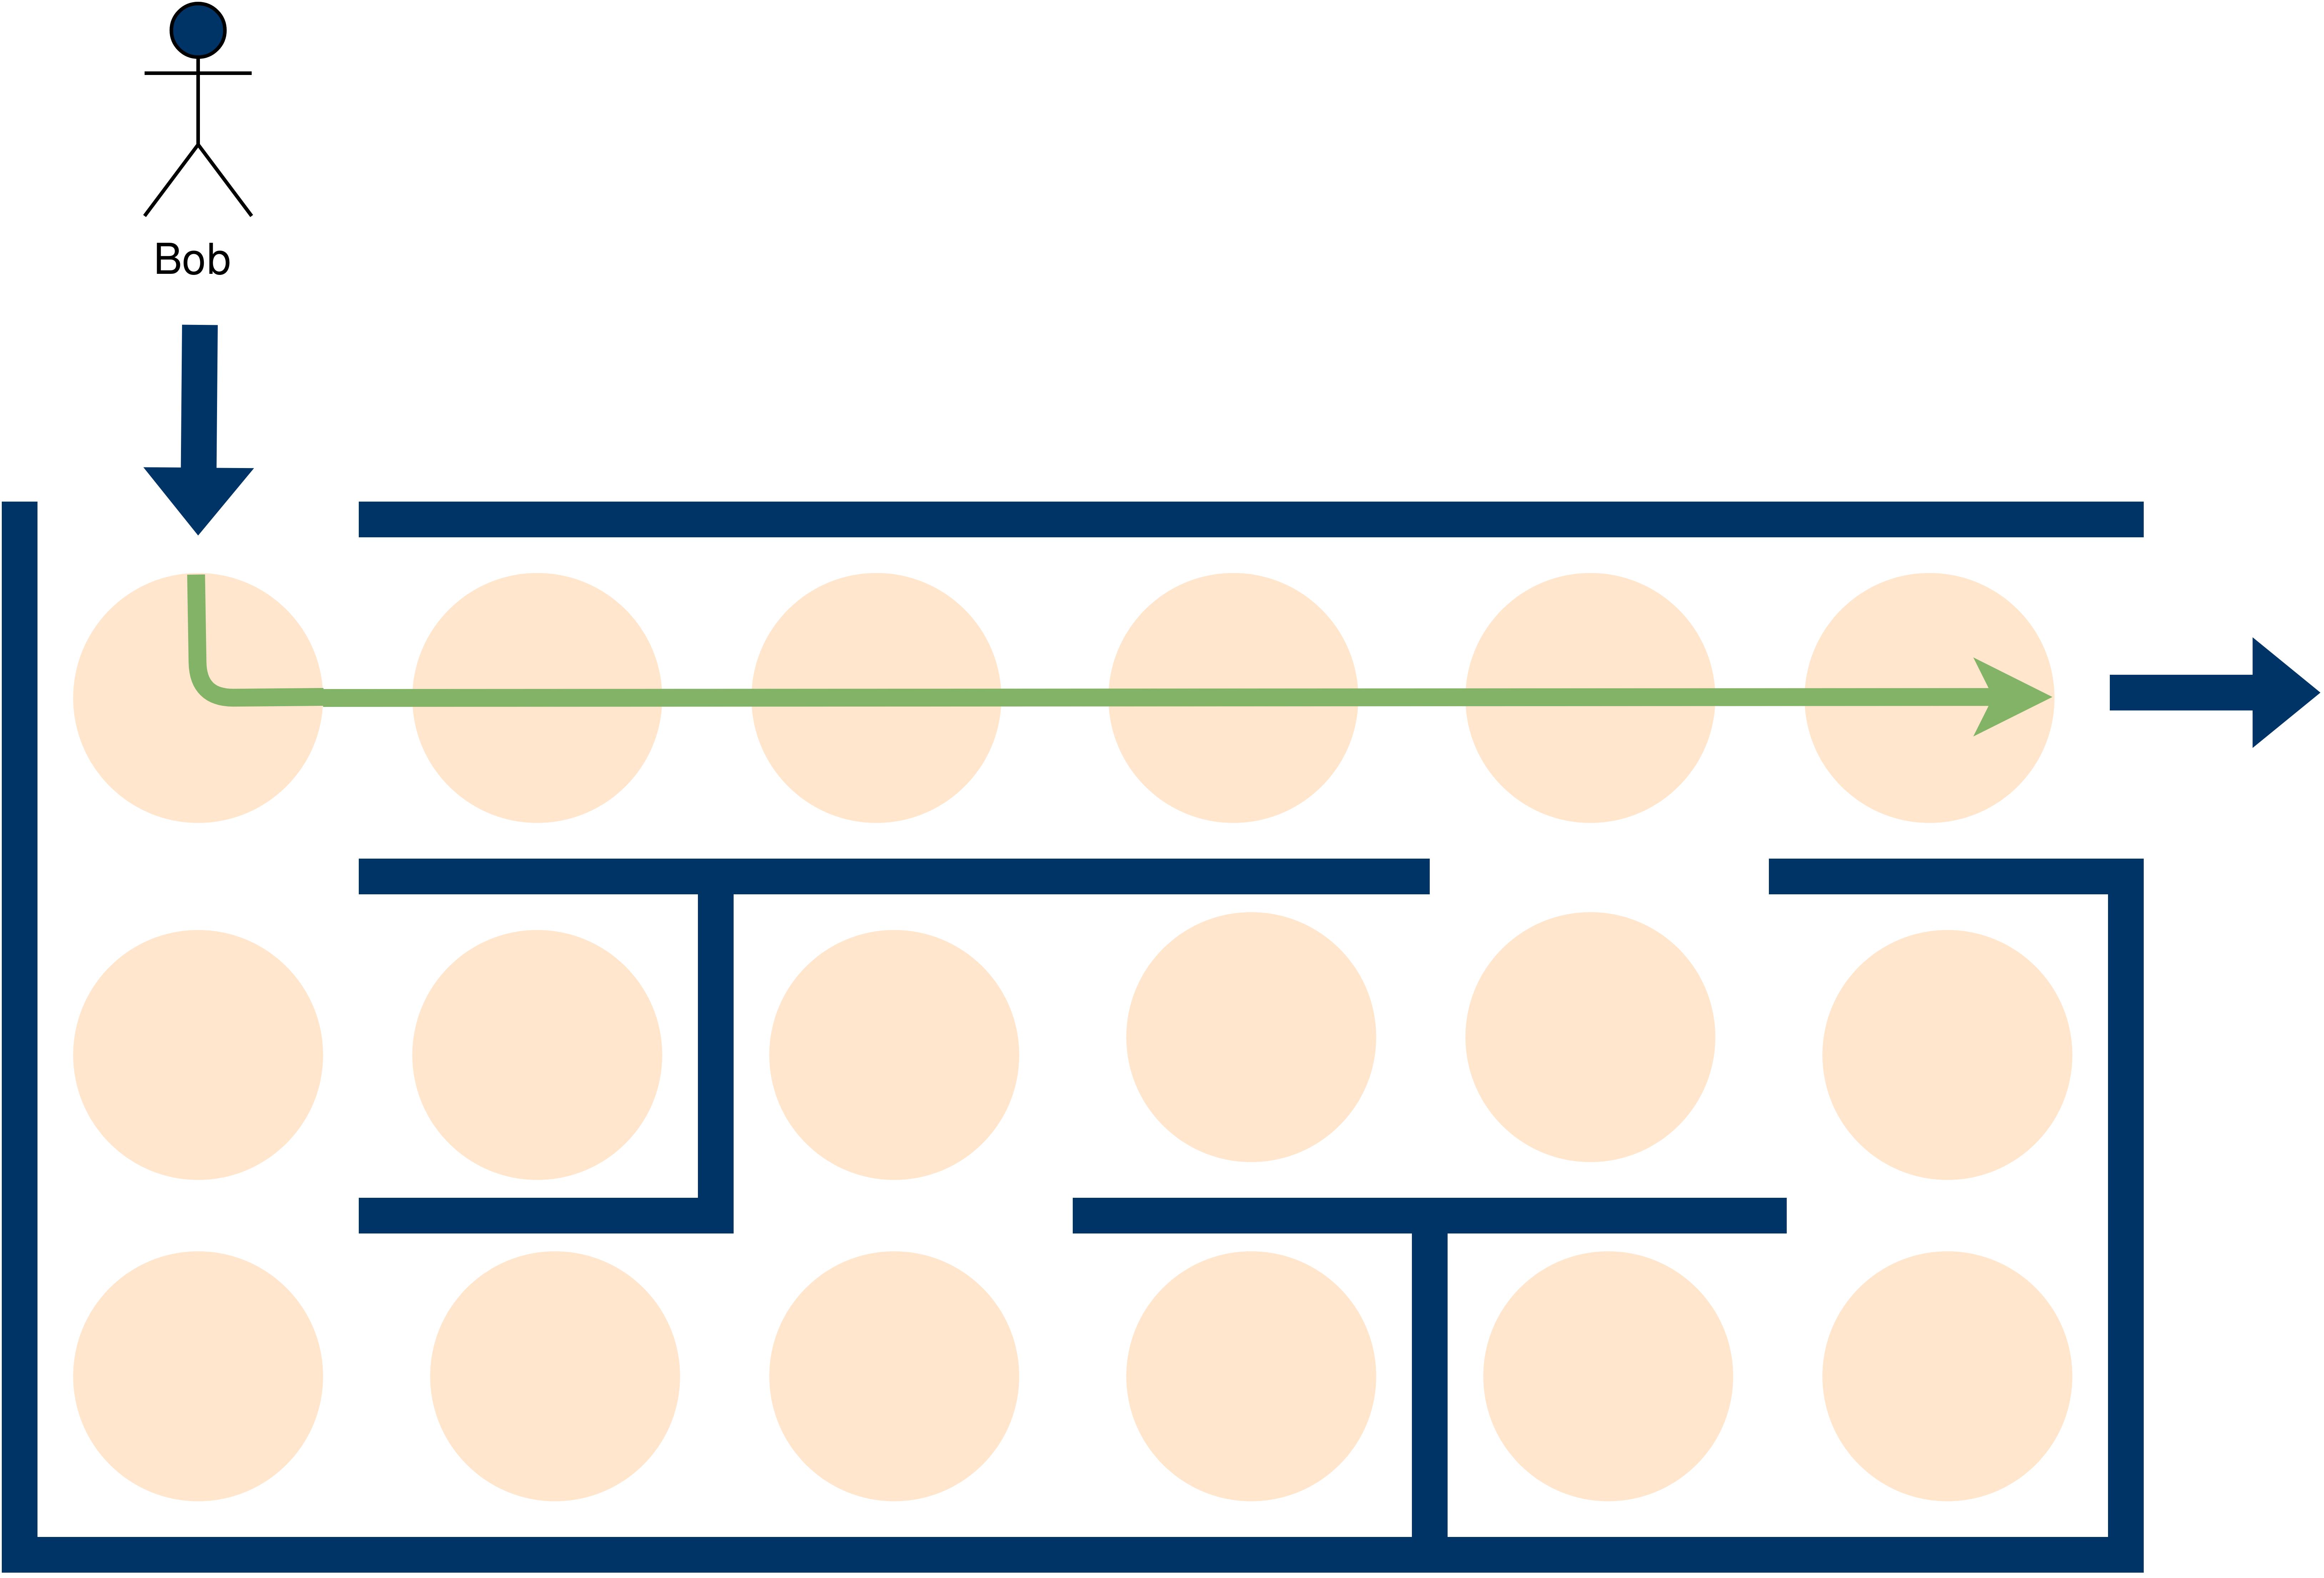
\includegraphics[width=0.7\textwidth]{../figures/GBeispiel1.png}
        \caption{der direkte Weg ist repräsentiert durch das Wort \alert{\MoveDown\Forward\Forward\Forward\Forward\Forward\Forward}}
    \end{figure}
    \end{alertblock}
\end{frame}
}  

{\setbeamercolor{palette primary}{bg=ExColor}
\begin{frame}{Lösung}
    \only<1>{
    \begin{figure}
        \centering
        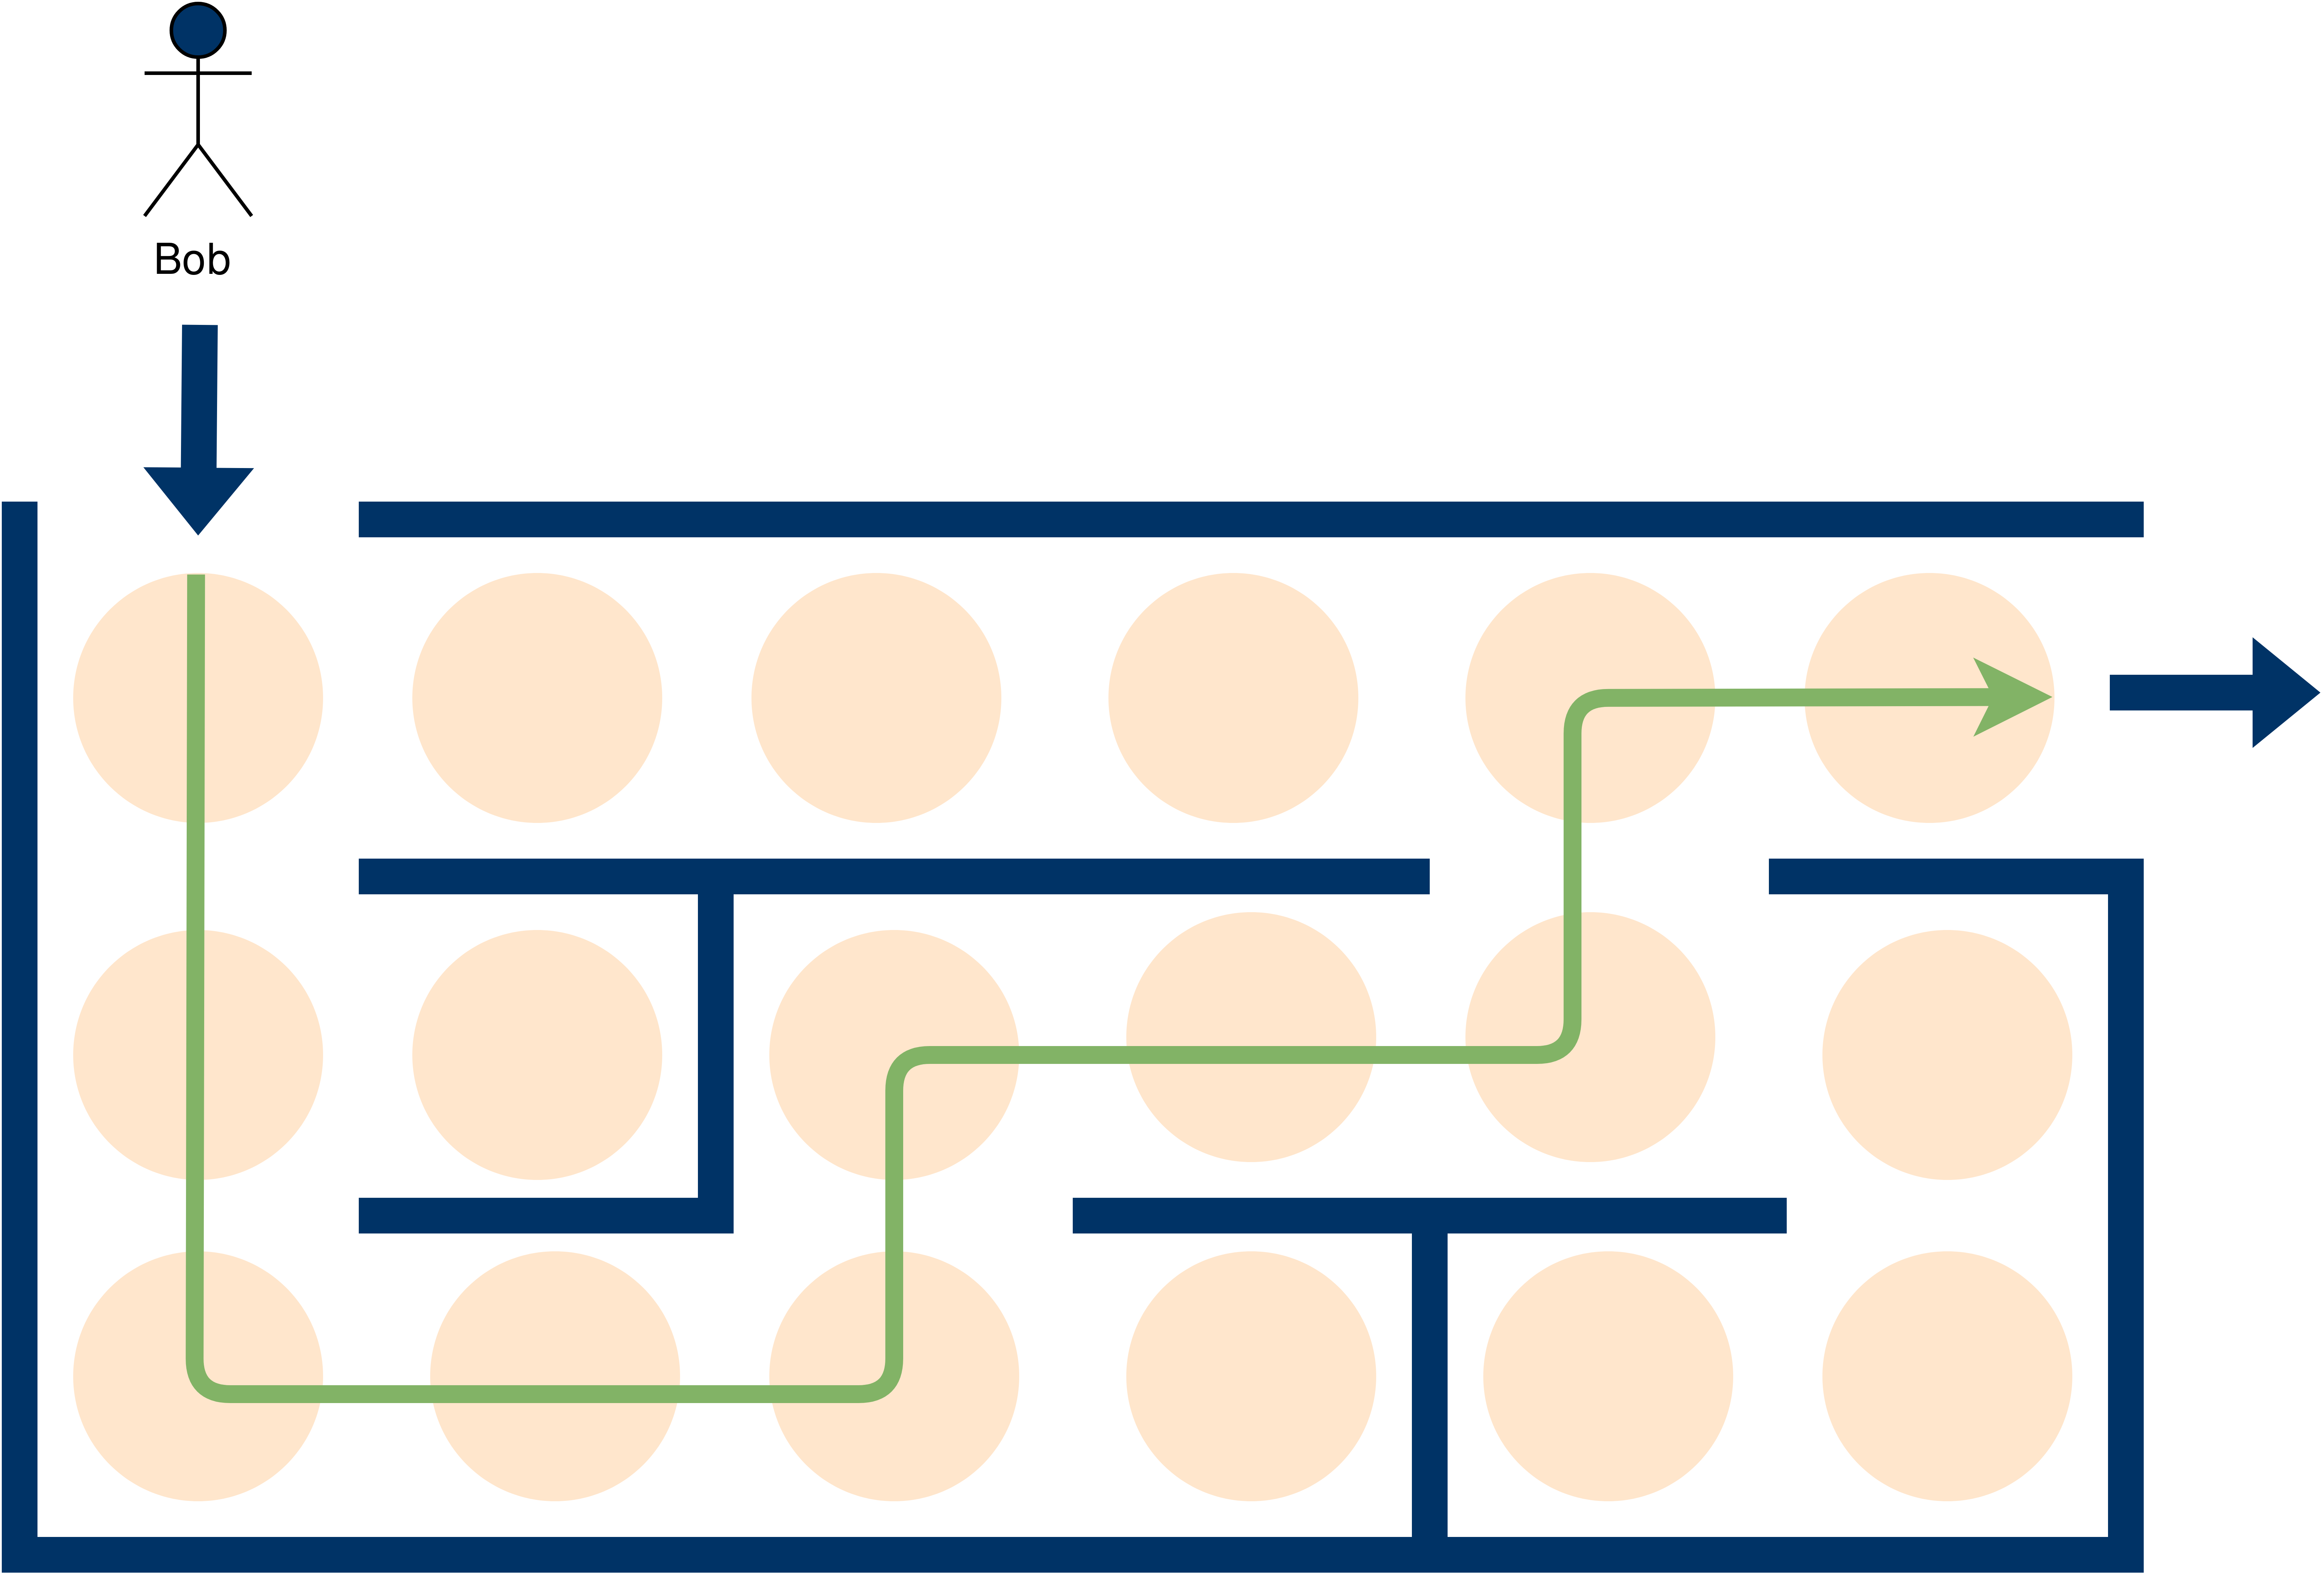
\includegraphics[width=0.7\textwidth]{../figures/GBeispiel2.png}
        \caption{Indirekter Weg}
        
    \end{figure}
    }
    \only<2>{
    \begin{figure}
        \centering
        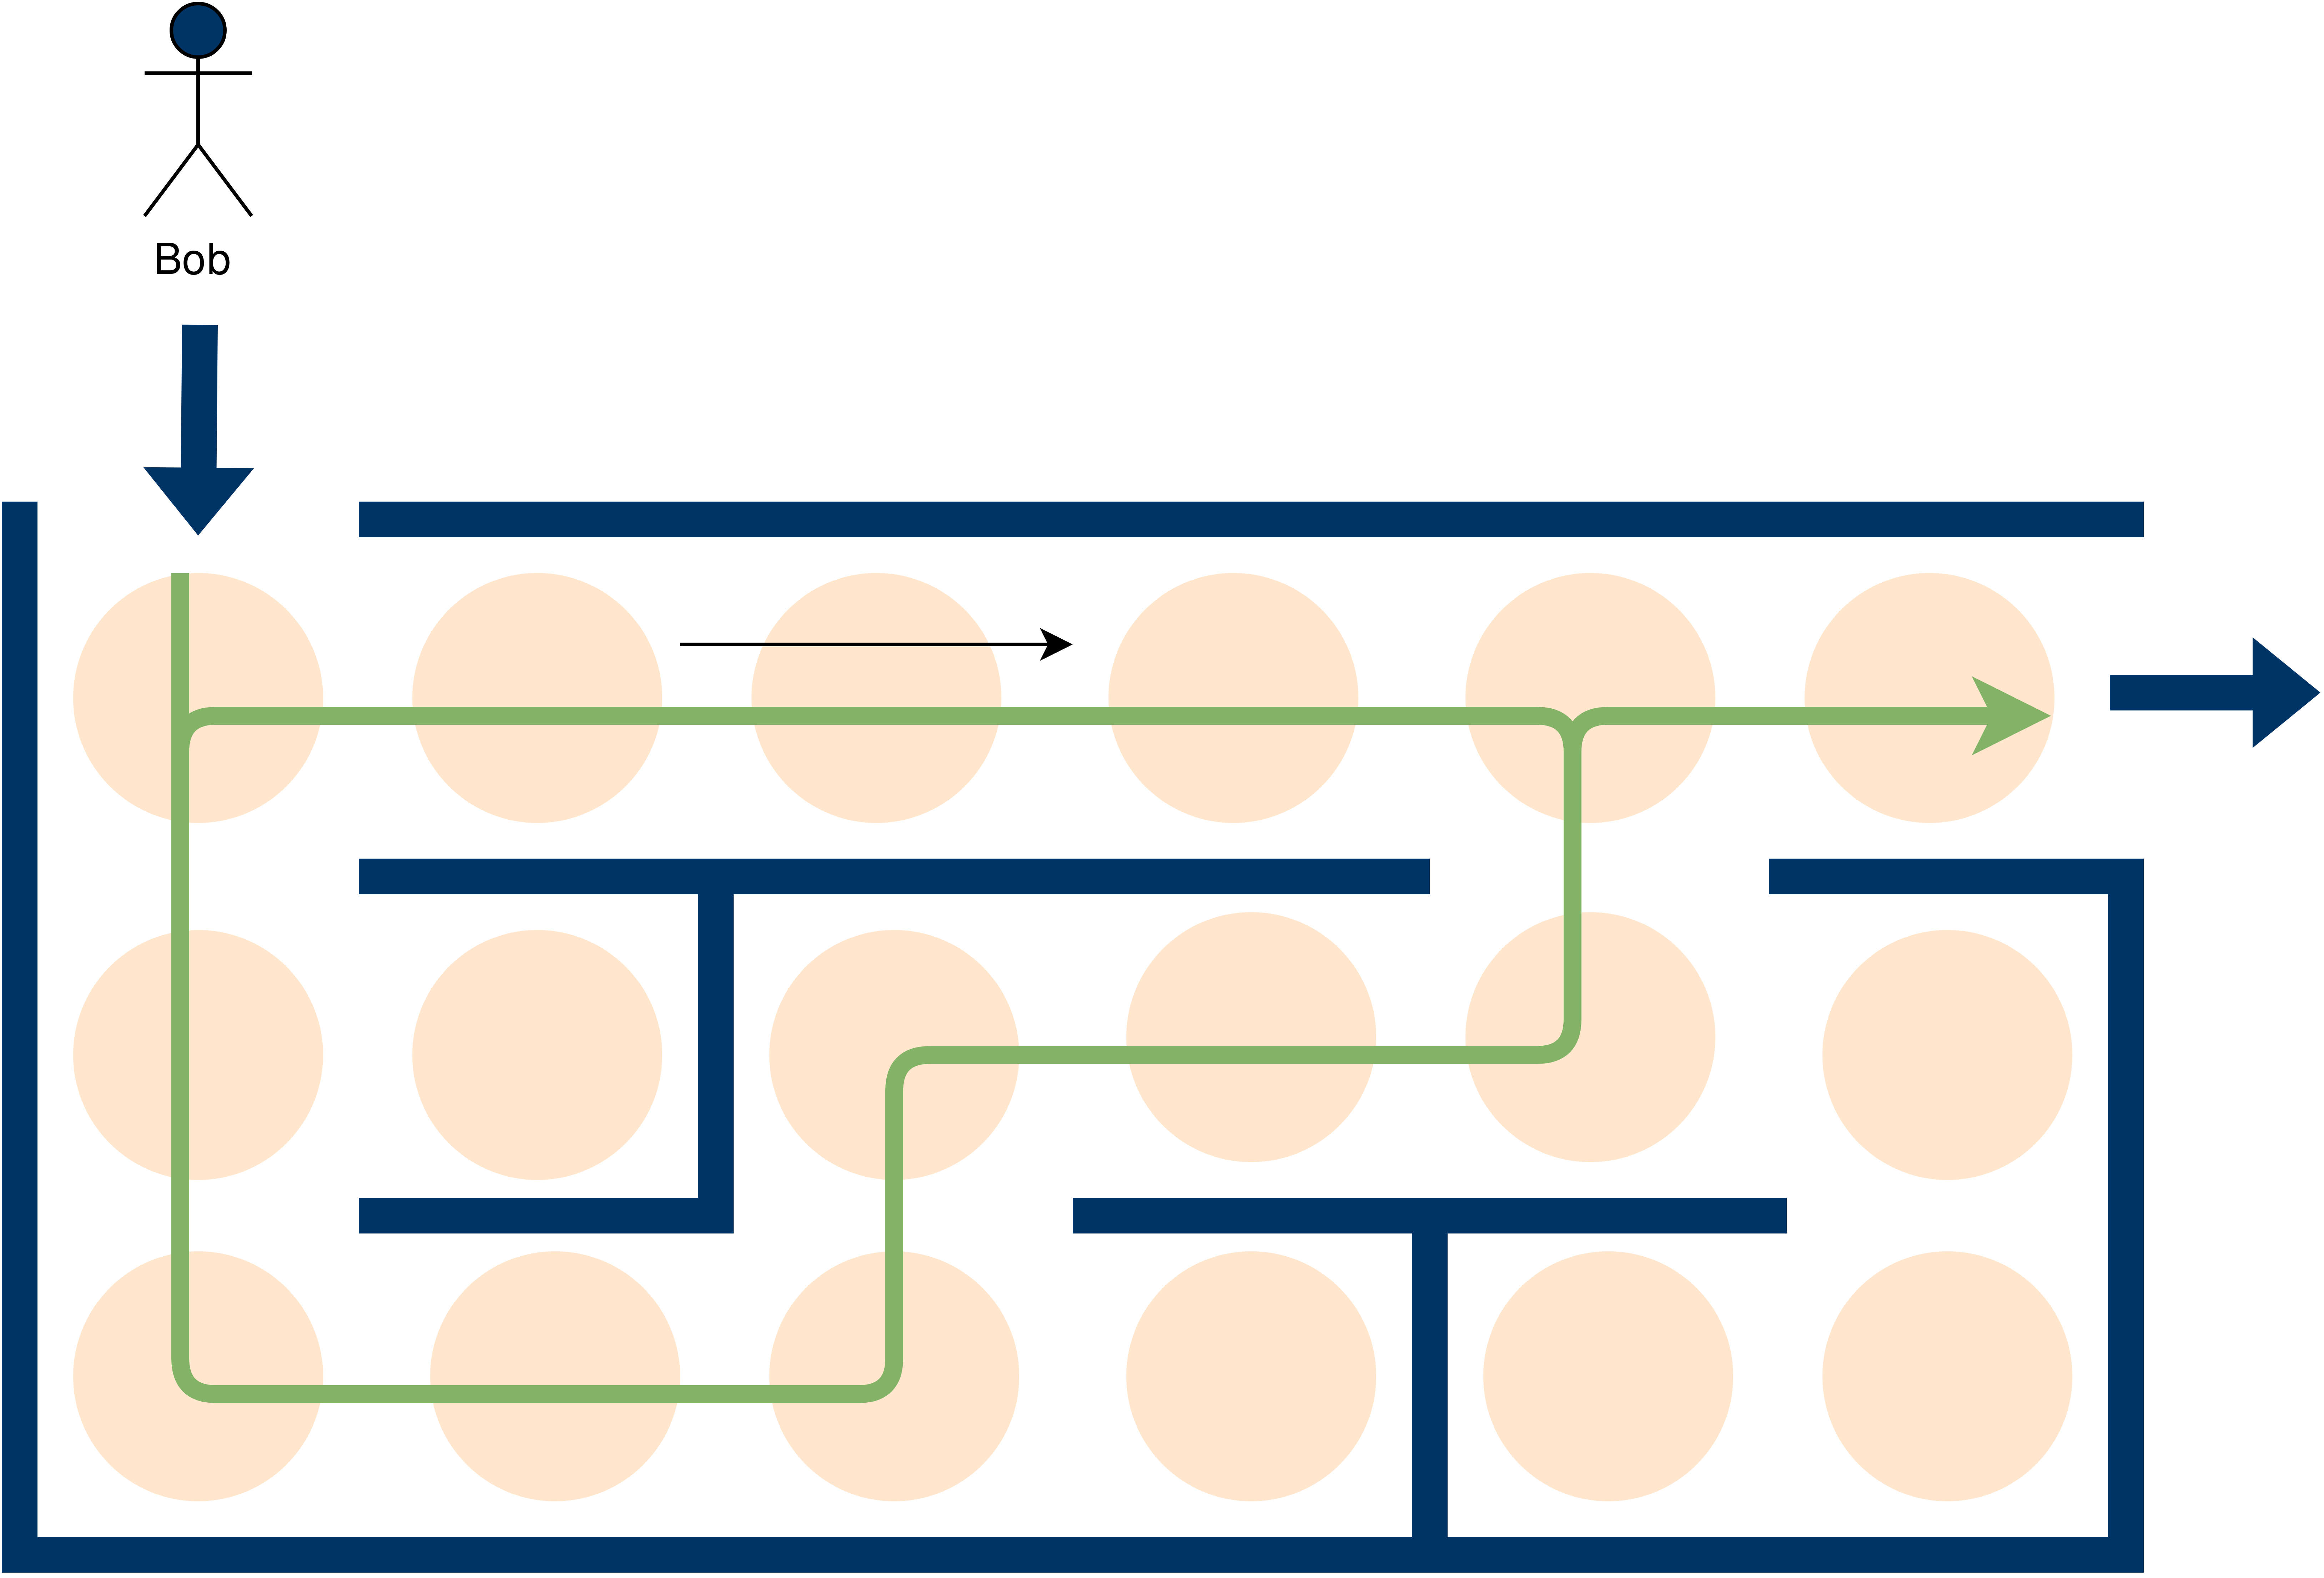
\includegraphics[width=0.7\textwidth]{../figures/GBeispiel3.png}
        \caption{Schlaufe Uhrzeigersinn}
        
    \end{figure}\textbf{}
    }
    \only<3>{
    \begin{figure}
        \centering
        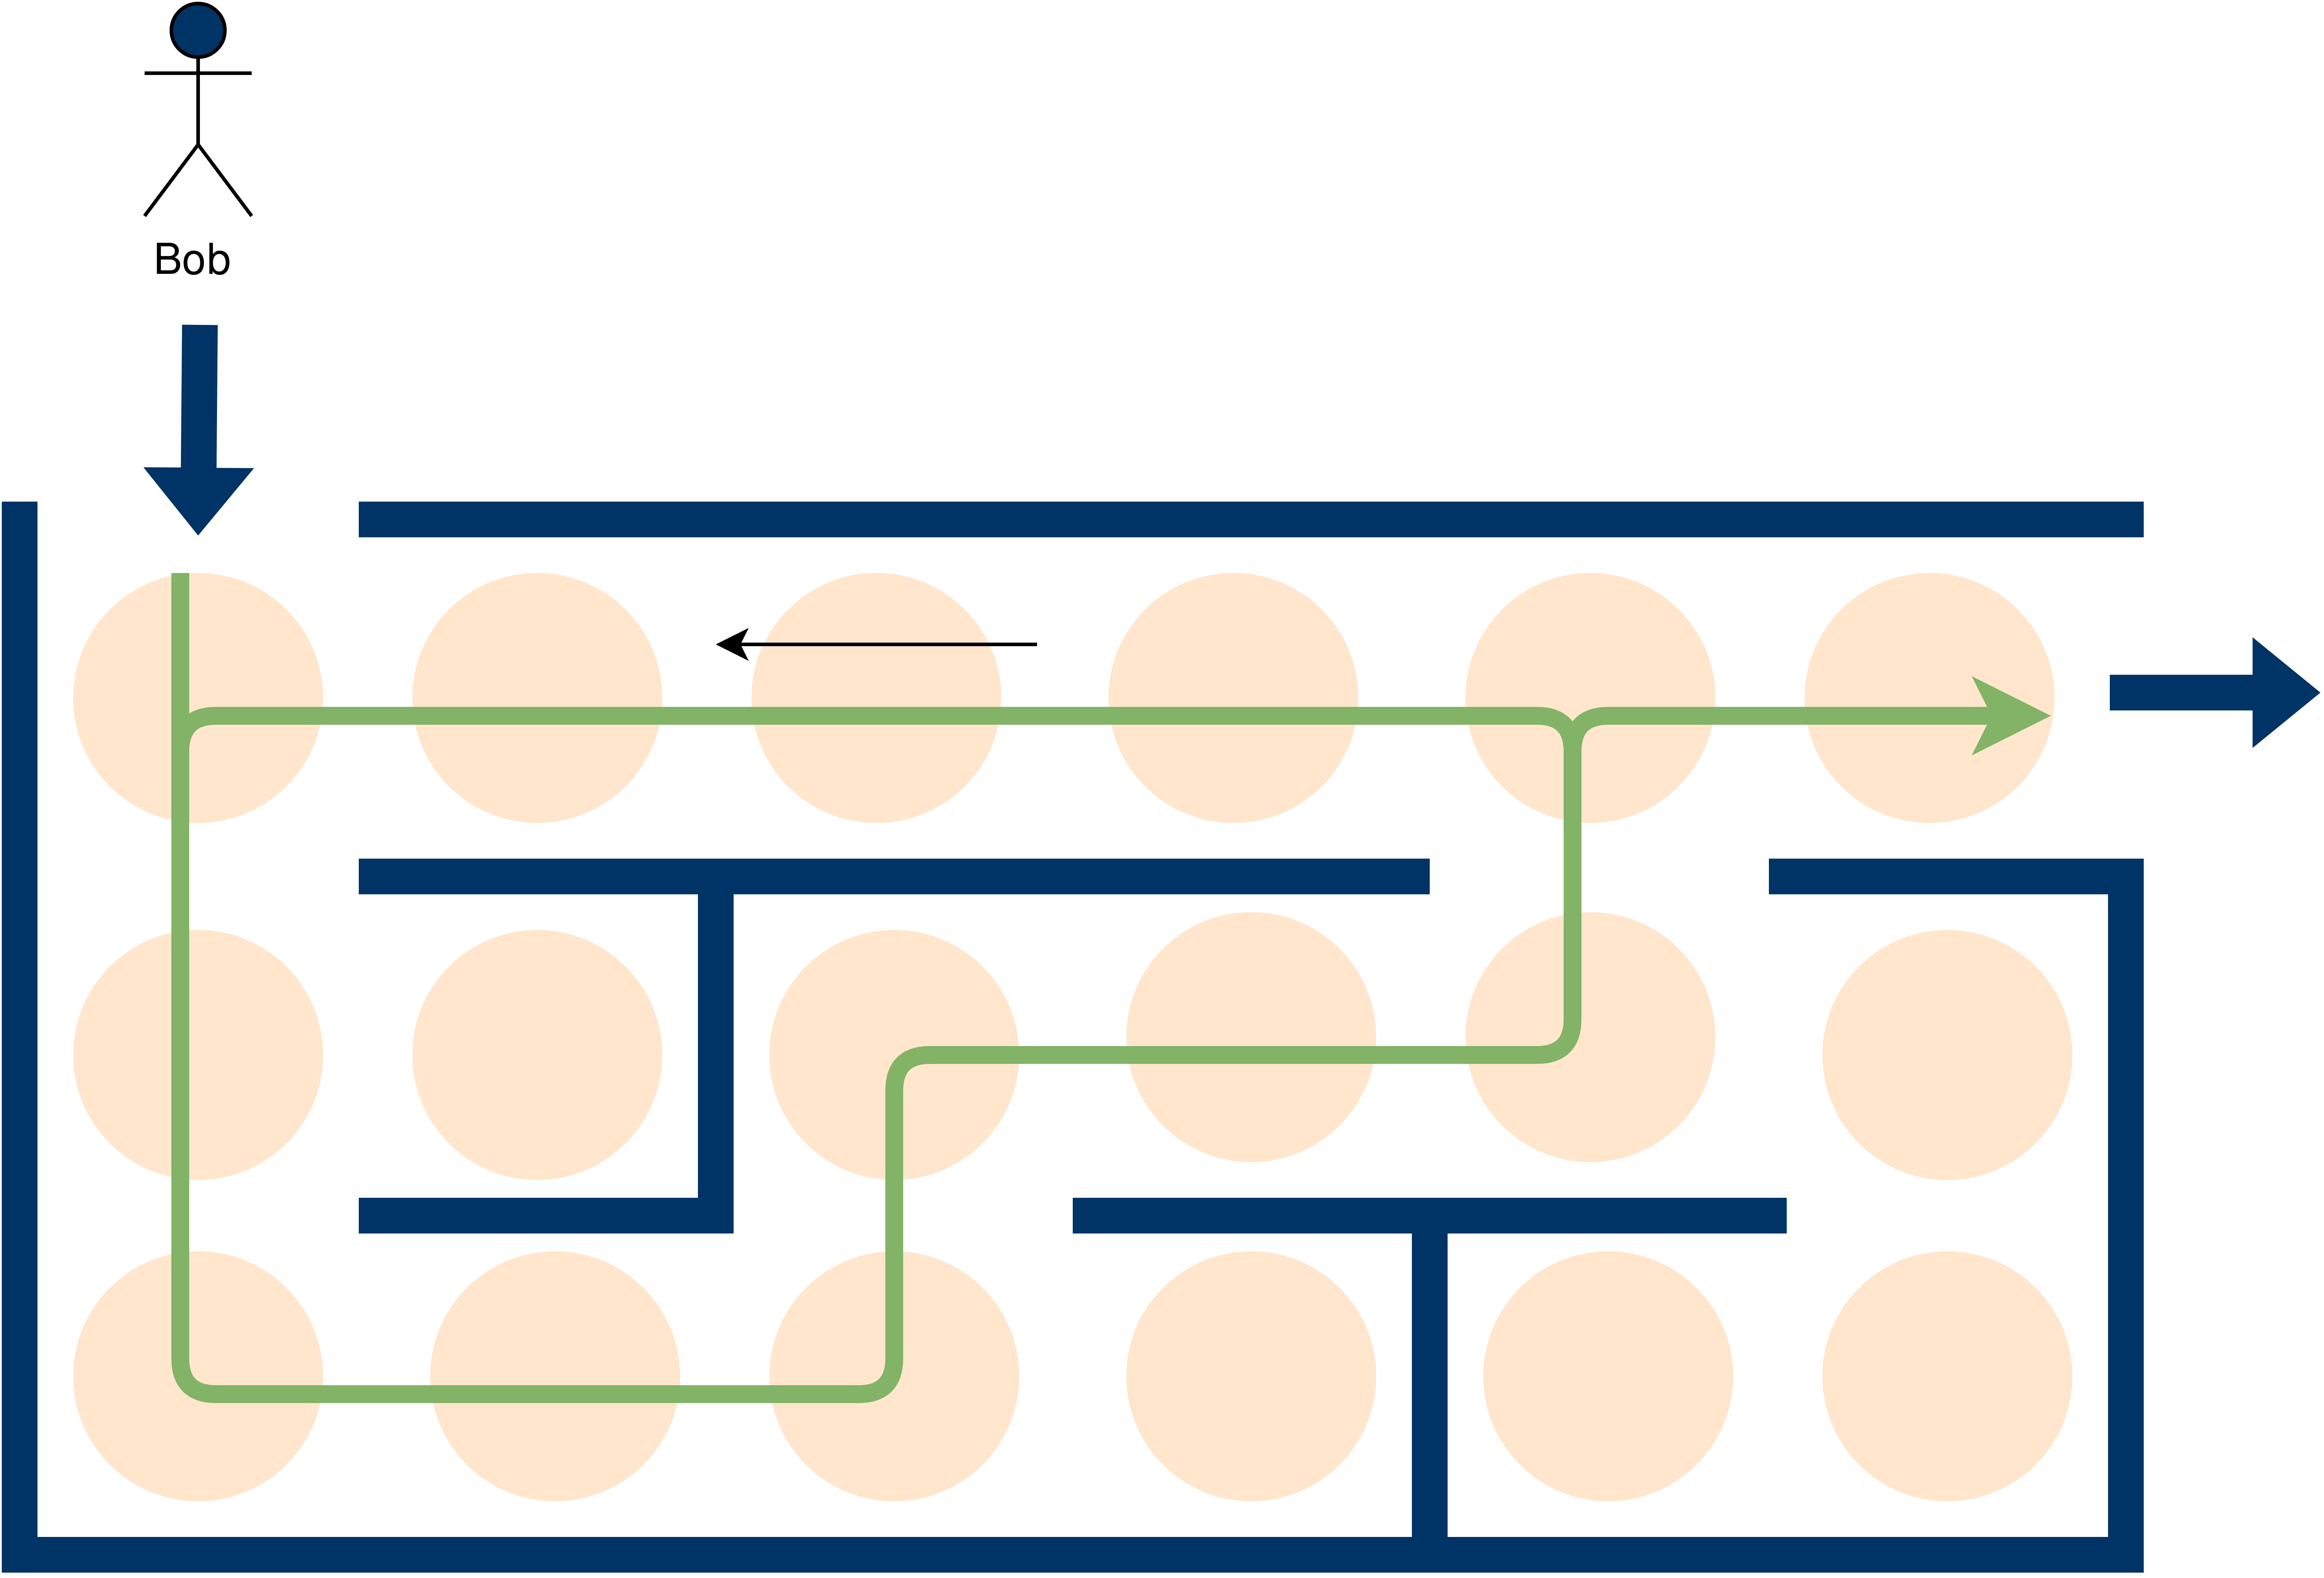
\includegraphics[width=0.7\textwidth]{../figures/GBeispiel4.png}
        \caption{Schlaufe gegen Uhrzeigersinn}
        
    \end{figure}
    }
\end{frame}
}

{\setbeamercolor{palette primary}{bg=ExColor}
\begin{frame}{Lösung}
    \begin{columns}
    \column{0.45\textwidth}
    \begin{alertblock}{Eine Möglichkeit:}
     %Wir nehmen uns zwei Variablen um zwischen den Einstiegsrichtungen zu unterscheiden für jeden Entscheidungspunkt und konstruieren damit  unsere Grammatik:\\
         $G = (V, \Sigma, P, S)$, wobei \\
         $V = \{S, A_u, A_r, B_u, B_l\}$ \\
         $\Sigma = \{\text{\Rewind, \MoveUp, \Forward, \MoveDown}\}$ \\
         $P = \{S \rightarrow \text\MoveDown A_u \mid \text\MoveDown A_r,$\\
         \qquad\; $A_u \rightarrow \text{\Forward\Forward\Forward\Forward} B_l$\\
         \qquad\; $A_r \rightarrow \text{\MoveDown\MoveDown\Forward\Forward\MoveUp\Forward\Forward\MoveUp} B_u,$\\
         \qquad\; $B_l \rightarrow \text{\MoveDown\Rewind\Rewind\MoveDown\Rewind\Rewind\MoveUp\MoveUp} A_u \mid \text{\Forward\Forward},$\\
         \qquad\; $B_u \rightarrow \text{\Rewind\Rewind\Rewind\Rewind} A_r \mid \text{\Forward\Forward}\}$
    \end{alertblock}
    \column{0.55\textwidth}
    \begin{figure}
        \centering
        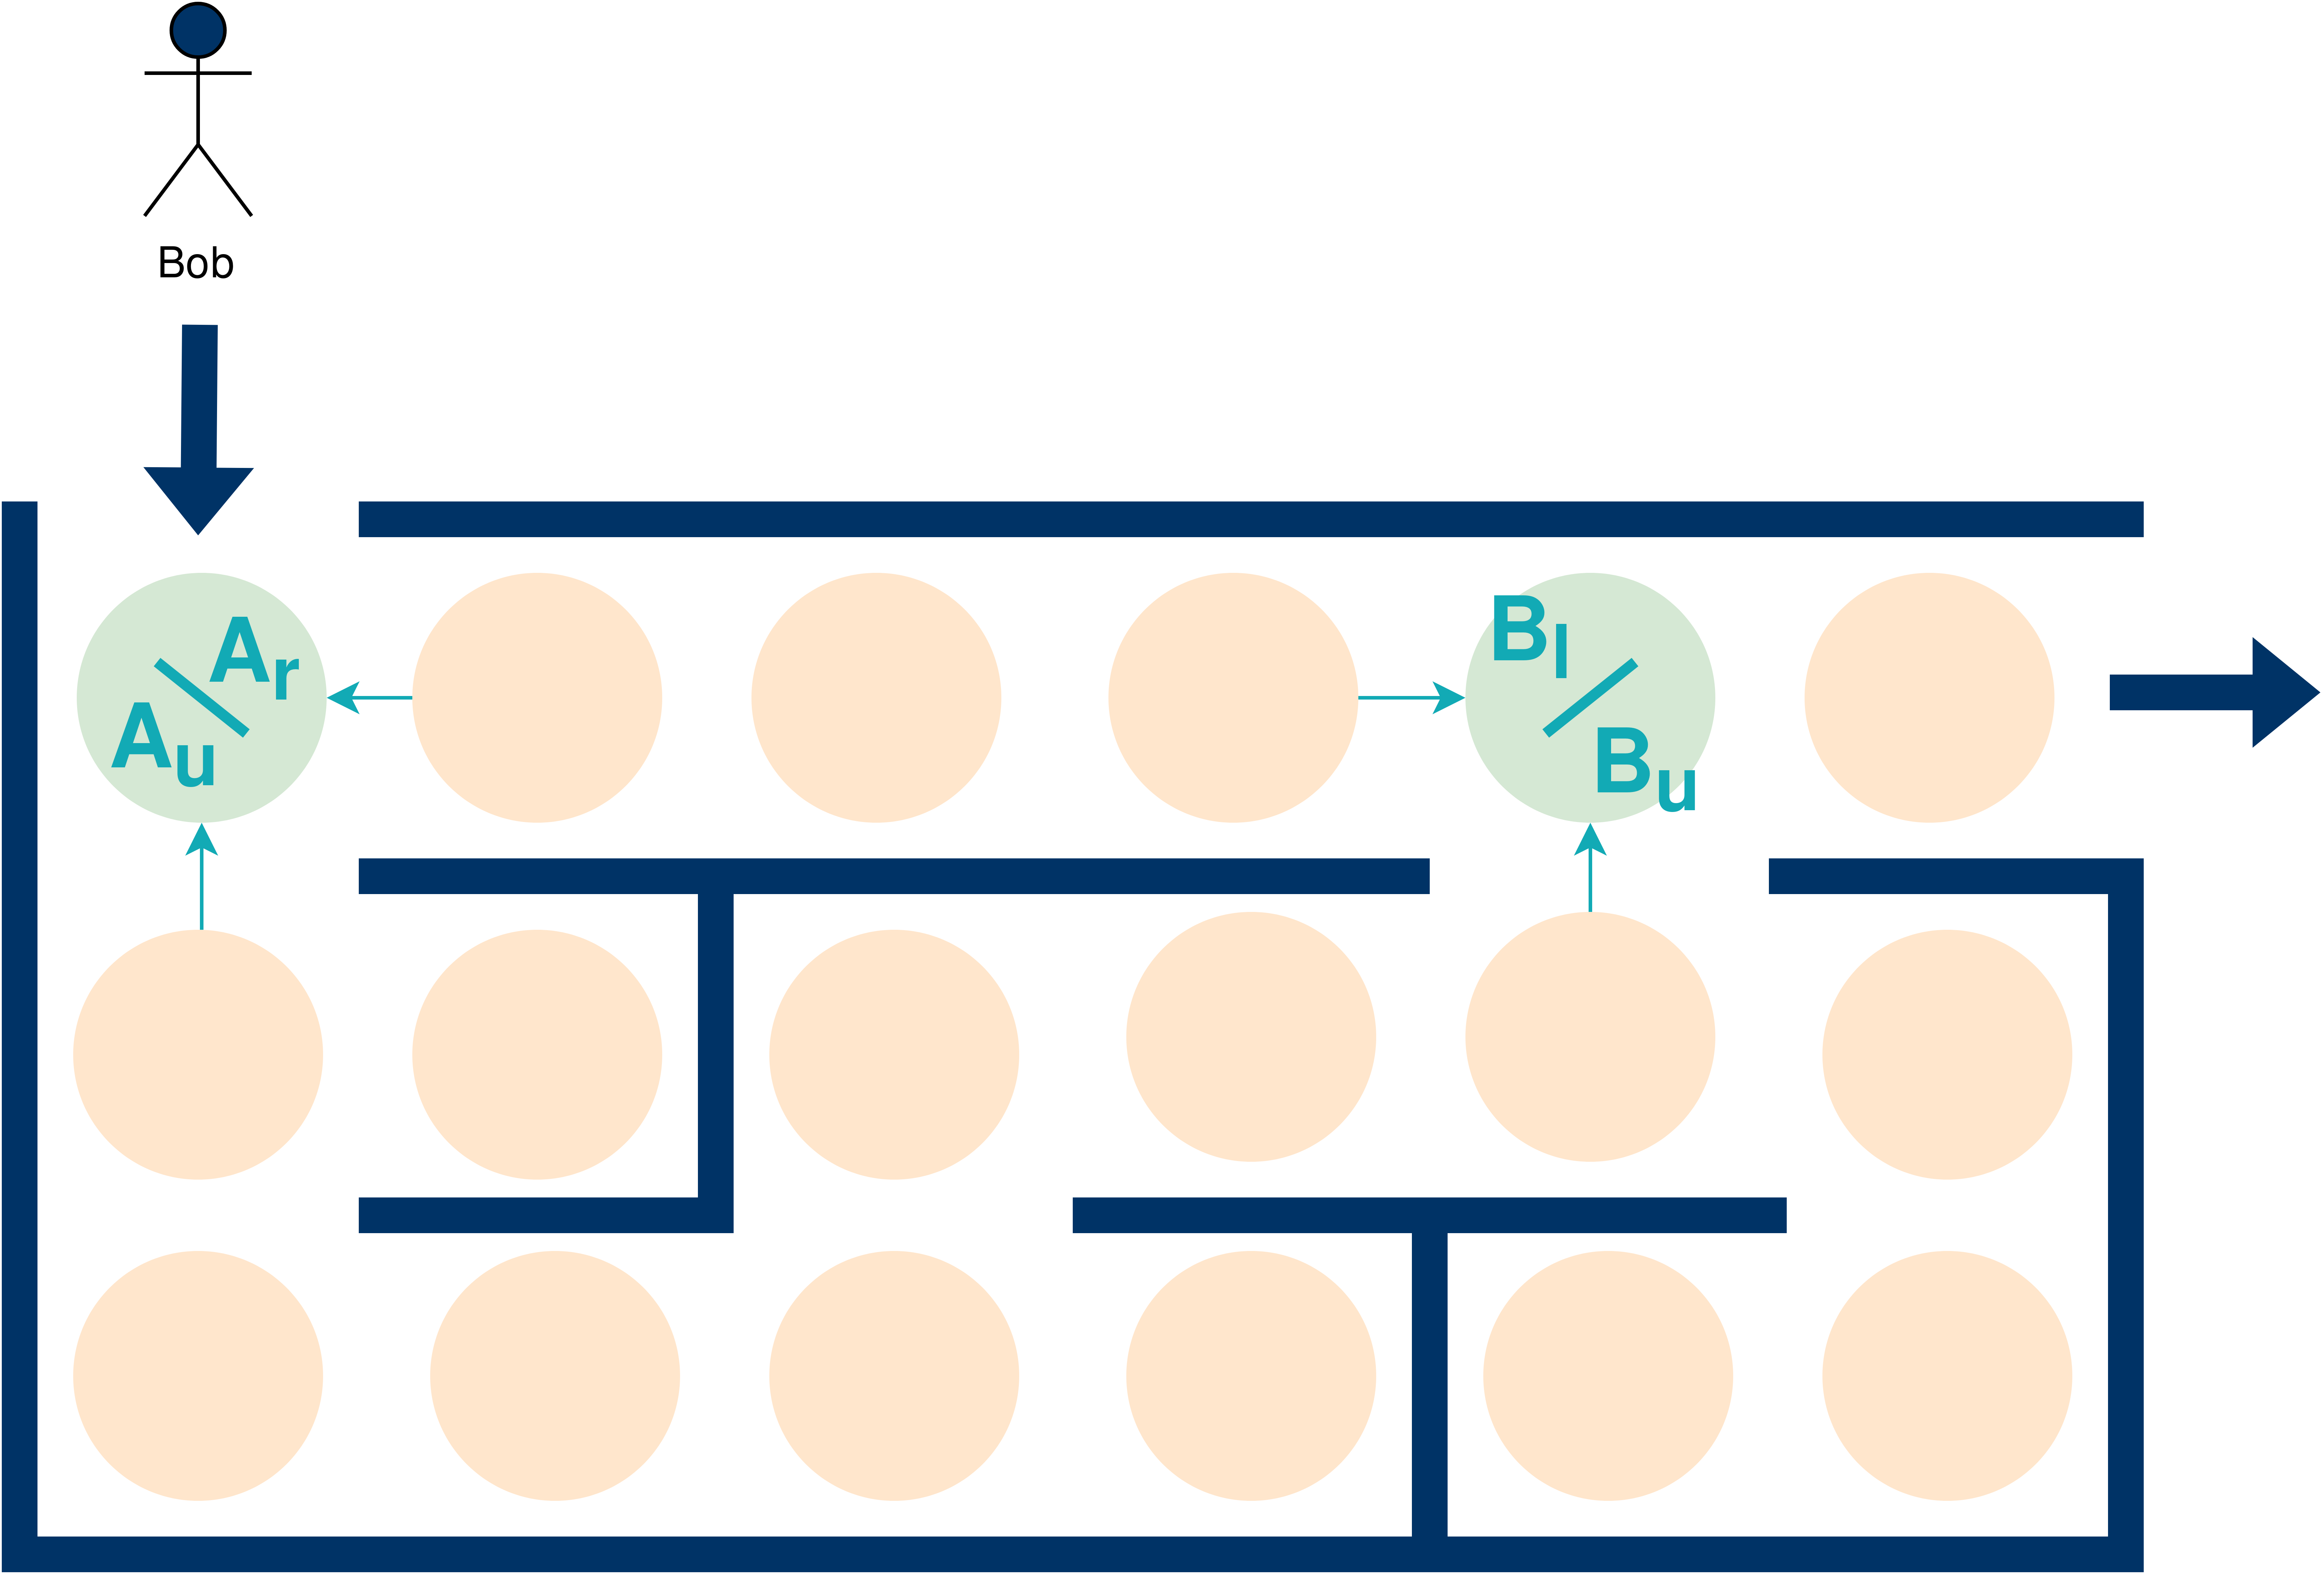
\includegraphics[width=0.9\textwidth]{../figures/GBeispielHowTo.png}
        \caption{Es muss unterschieden werden, ob Bob von links, rechts oder unten kam}
        
    \end{figure}
    \end{columns}
    \small\emph{Erinnerung:} Bob kann nicht auf ein Feld zurücktreten von dem er gerade kam
\end{frame}
} 

\subsubsection{Ableiten}
\begin{frame}[fragile]{Ableiten}
    Wir können durch das Ableiten formal zeigen, dass ein Wort von einer Grammatik erzeugt wird.\\
    \small{Wir betrachten L = \{$ww^R\;|\;w^R\text{ ist w rückwärts, }w \in \{a, b\}^n, n>0, n\in \mathbb{N}$\}\\
    mit der Grammatik $G=(V,\Sigma,P,S)$, wobei\\
    $V=\{S\}$, $\Sigma=\{a,b\}$, $P = \{S \rightarrow aSa \mid bSb \mid aa \mid bb$\}}
    \metroset{block=fill}
    \begin{exampleblock}{Beipspiel}
        Wir zeigen $ww^R = ababbbbaba \in$ L.\\
        \small{$S\Rightarrow_G aSa \Rightarrow_G abSba \Rightarrow_G  abaSaba \Rightarrow_G ababSbaba$ \\ $\Rightarrow_G ababbbbaba$}\\\qed
    \end{exampleblock}
\end{frame}

{\setbeamercolor{palette primary}{bg=ExColor}
\begin{frame}{Denkpause}
    \begin{alertblock}{Aufgaben}
    Zeige.
    \end{alertblock}
    \metroset{block=fill}
    \begin{block}{Normal}
    \begin{itemize}
        \item $P_1=\{S\rightarrow aaS\;|\;\emptyWord\}$ erzeugt $aaaa$
        \item $P_2=\{S\rightarrow AB$, $A\rightarrow aAb \;|\; ab\; |\;\emptyWord$, $B\rightarrow cB \;|\; \emptyWord\}$ erzeugt $aabbc$
        \item $P_3=\{S\rightarrow UV$, $U\rightarrow aU \;|\; bU \; |\; \emptyWord$, $V\rightarrow c \;|\; d\}$ erzeugt $abac$
        \item $P_4=\{S\rightarrow XXX$, $X\rightarrow a \;|\; b \;|\; c\}$ erzeugt $aac$
    \end{itemize}
    \end{block}
    \begin{block}{Etwas Schwerer}
    \begin{itemize}
        \item $P_5=\{S\rightarrow a \;|\; aaaS\}$ erzeugt $aaaa$
        \item $P_6=\{S\rightarrow AAAB$, $AB\rightarrow BA, 
        A\rightarrow cA \;|\; Ac \;|\; a, 
        B\rightarrow cB \;|\; Bc \;|\; b\}$ erzeugt $cabcacca$
        \item $P_7=\{S\rightarrow U\text{\Stopsign} \;|\; \text{\Stopsign}$, $U\rightarrow \text{\Rewind} U \;|\; \text{\MoveUp} U \;|\; \text{\Forward} U \;|\; \text{\MoveDown} U \;|\;\emptyWord\}$ erzeugt \Forward\Stopsign
    \end{itemize}
    \end{block}
\end{frame}
}

{\setbeamercolor{palette primary}{bg=ExColor}
\begin{frame}{Lösungen}
Alle Lösungen sind Beispiellösungen, es sind auch andere möglich.
    \begin{itemize}[<+- | alert@+>]
        \item $S\Rightarrow_G aaS \Rightarrow_G aaaaS \Rightarrow_G aaaa$
        \item $S\Rightarrow_G AB \Rightarrow_G aAbB \Rightarrow_G aabbB \Rightarrow_G aabbcB \Rightarrow_G aabbc$
        \item $S\Rightarrow_G UV \Rightarrow_G aUV \Rightarrow_G abUB \Rightarrow_G abaUB \Rightarrow_G abaB \Rightarrow_G abac$
        \item $S\Rightarrow_G XXX \Rightarrow_G aXX \Rightarrow_G aaX \Rightarrow_G aac$
        \item $S\Rightarrow_G aaaS \Rightarrow_G aaaa$
        \item $S\Rightarrow_G AAAB \Rightarrow_G AABA \Rightarrow_G ABAA \Rightarrow_G cABAA \Rightarrow_G caBAA \Rightarrow_G cabAA \Rightarrow_G cabcAA \Rightarrow_G cabcaA\Rightarrow_G cabcacA \Rightarrow_G cabcaccA \Rightarrow_G cabcacca$
        \item $S\Rightarrow_G U\text{\Stopsign} \Rightarrow_G \text{\Forward}U\text{\Stopsign} \Rightarrow_G \text{\Forward}\text{\Stopsign}$
    \end{itemize}
\end{frame}
}  


\section{Wiederholung}
\begin{frame}[fragile]{Das können wir jetzt beantworten}
	\begin{alertblock}{Vollständige Induktion}
		\begin{itemize}
			\item Was ist die Idee der Induktion?
			\item Welche Schritte hat die Induktion? %IA,IV,IS
			\item Für welche Aussagen ist die Induktion geeignet?
		\end{itemize}
	\end{alertblock}
\end{frame}

\begin{frame}[fragile]{Das können wir jetzt beantworten}
	\begin{alertblock}{Grammatiken}
		\begin{itemize}
        	\item Was sind Grammatiken?
			\item Was ist der Zusammenhang zwischen Grammatiken und Sprachen?
			\item Was sind Nichtterminale?
			\item Was sind Terminale?
			\item Bilden einer Grammatik für gegebene Sprache
        	\item Wie finde ich raus, ob ein Wort von einer Grammatik erzeugt wird?
		\end{itemize}
	\end{alertblock}
\end{frame}

\begin{frame}[standout]
  Noch Fragen?
\end{frame}

\begin{frame}[fragile]{Glossar}
    \small
    \begin{tabular}{p{0.12\textwidth} p{0.23\textwidth} p{0.5\textwidth}}
    \toprule
    Abk.&Bedeutung&Was?!\\
    \midrule
        $A \subseteq B$ & Teilmenge & Alle Elemente aus A sind auch in B enthalten. Dabei können die Mengen auch gleich sein.\\
        $A \subsetneq B$ & echte Teilmenge & Alle Elemente aus A sind auch in B enthalten. Jedoch enthält B noch Elemente, die nicht in A enthalten sind.
        $\implies$ Mengen sind nicht gleich!\\
        $A \subset B$ & Teilmenge \emph{oder} echte Teilmenge & Bei manchen Leuten $\subseteq$, bei manchen $\subsetneq$. Mehrdeutig, lieber nicht verwenden!\\
    \bottomrule
    \end{tabular}
\end{frame}


% \section{Wiederholung}

% \begin{frame}[fragile]{Das können wir jetzt beantworten}
%     \blindtext
% \end{frame}

% \begin{frame}[standout]
%   Noch Fragen?
% \end{frame}

% \begin{frame}[fragile]{Glossar}
%     \small
%     \begin{tabular}{p{0.05\textwidth} p{0.25\textwidth} p{0.5\textwidth}}
%     \toprule
%     Abk.&Bedeutung&Was?!\\
%     \midrule
%         gdw.&genau dann wenn&Äquivalenz zwischen Aussagen\\
%         $\mathbb{N}$&natürliche Zahlen (mit 0)&In der theoretischen Informatik enthält $\mathbb{N}$ die 0: $\mathbb{N}=\{0,1,2,3,\dots\}$\\
%         \Sigma & Sigma& mit diesem Zeichen wird oft das Alphabet (die Menge an verwendbaren Symbolen) repräsentiert\\
%         $\Sigma^\ast$&Sigma Stern&Menge aller Möglichkeiten Elemente aus $\Sigma$ hintereinander zu schreiben\\
%     \bottomrule
%     \end{tabular}
% \end{frame}


\end{document}
